
\subsection{Tables and Graphs}
\label{lemma:tables and graphs}

{\color {red}CW: I put some tables and graphs here.}

{\color {red}CW: We should make agreement about the interface.}

\autoref{fig:crdt-implementaton of this paper, their correctness, and their interface} gives the \crdtimp{} proved in our work, their correctness, and their interface (methods).

% \begin{figure}[t]
% %\centering

% \begin{tabular}{|l|c|r|}
% \hline
% \crdtimp&Correctness&Interface\\
% \hline
% counter~\cite{ShapiroPBZ11}&\tzerolin&$\alabelshort[{\tt inc}]{}$, $\alabelshort[{\tt dec}]{}$\\
% \hline
% PN-counter~\cite{ShapiroPBZ11}&\tzerolin&$\alabelshort[{\tt inc}]{}$, $\alabelshort[{\tt dec}]{}$\\
% \hline
% LWW-register~\cite{DBLP:journals/rfc/rfc677}&\tonelin&$\alabelshort[{\tt write}]{value}$, $\alabellong[{\tt read}]{}{value}{}$\\
% \hline
% Multi-value register~\cite{DBLP:conf/sosp/DeCandiaHJKLPSVV07}&\tzerolin&$\alabelshort[{\tt write}]{value}$, $\alabellong[{\tt read}]{}{Set \ value}{}$\\
% \hline
% 2P-set~\cite{ShapiroPBZ11}&\tzerolin&$\alabelshort[{\tt add}]{value}$, $\alabelshort[{\tt remove}]{value}$, $\alabellong[{\tt read}]{}{Set \ value}{}$\\
% \hline
% LWW-set~\cite{ShapiroPBZ11}&\tonelin&$\alabelshort[{\tt add}]{value}$, $\alabelshort[{\tt remove}]{value}$, $\alabellong[{\tt read}]{}{Set \ value}{}$\\
% \hline
% %PN-set~\cite{ShapiroPBZ11}&not \crdtlinearizable{}&$add$, $remove$, $read$\\
% %\hline
% OR-set~\cite{ShapiroPBZ11}&\tzerolin&$\alabelshort[{\tt add}]{value}$, $\alabelshort[{\tt remove}]{value}$, $\alabellong[{\tt read}]{}{Set \ value}{}$\\
% \hline
% RGA~\cite{RohJKL11}&\tonelin&$\alabelshort[{\tt addAfter}]{value,value}$, $\alabelshort[{\tt remove}]{value}$,
%                 \\ & & $\alabellong[{\tt read}]{}{List \ value}{}$\\
% \hline
% Wooki~\cite{DBLP:conf/wise/WeissUM07}&\tzerolin&$\alabelshort[{\tt addBetween}]{value,value,value}$, $\alabelshort[{\tt remove}]{value}$,
%                 \\ & & $\alabellong[{\tt read}]{}{List \ value}{}$\\
% \hline
% Treedoc~\cite{DBLP:conf/icdcs/PreguicaMSL09}&\tzerolin&$\alabelshort[{\tt addBetween}]{value,value,value}$, $\alabelshort[{\tt remove}]{value}$,
%                 \\ & & $\alabellong[{\tt read}]{}{List \ value}{}$\\
% \hline
% \end{tabular}

% \caption{\crdtimp{} of this paper, their correctness, and their interface.}
% \label{fig:crdt-implementaton of this paper, their correctness, and their interface}
% \end{figure}


% \autoref{fig:an example run of semantics} gives a example of two step of transitions on semantics of RGA. The first step is to do downstream of a $addAfter$, while the second step is to do operation $remove$. Here we can see that, the downstream of $addAfter$ always insert a new node into the Ti-tree $N$, while the downstream of $remove$ always insert a value into $Tomb$.

% \begin{figure}[t]
%   \centering
%   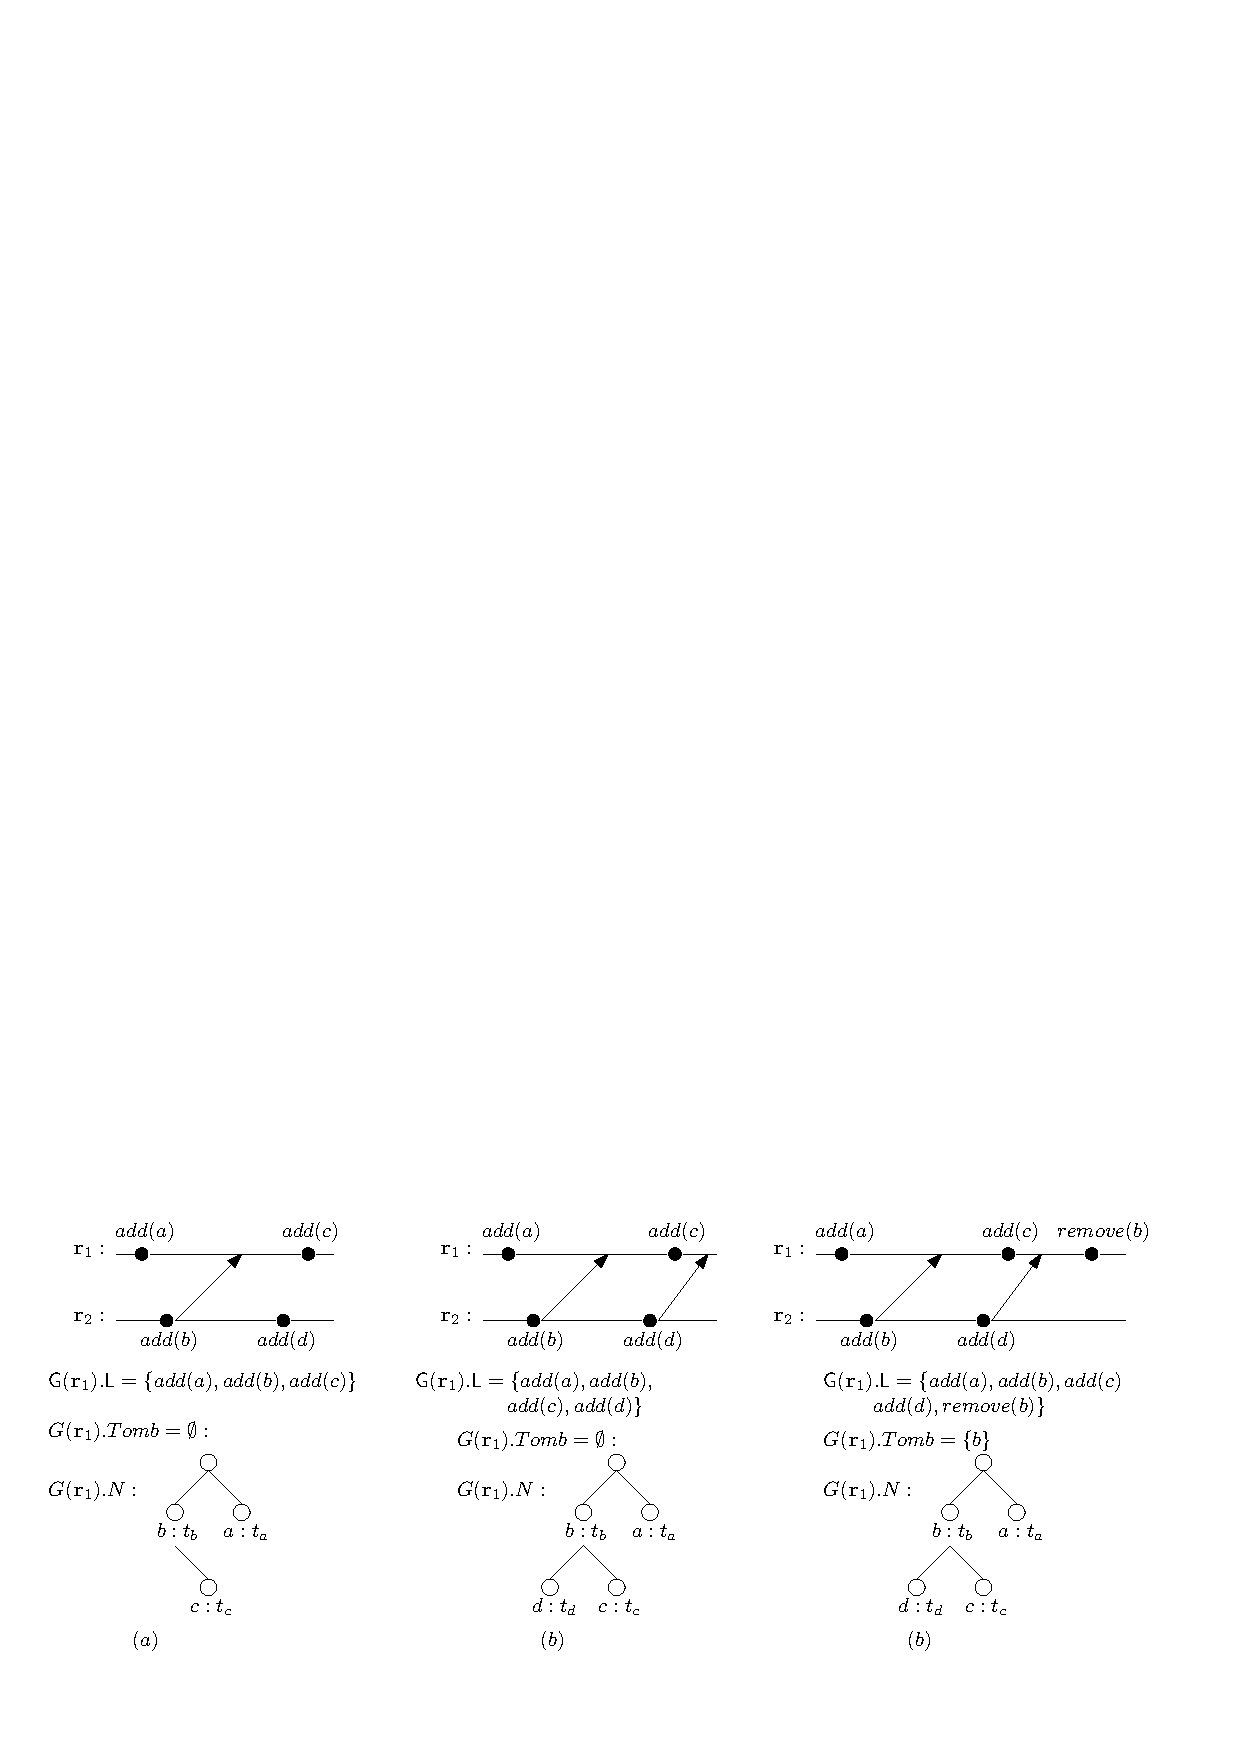
\includegraphics[width=1 \textwidth]{figures/ExplainSemantics.pdf}
% \vspace{-10pt}
%   \caption{An example run of semantics.}
%   \label{fig:an example run of semantics}
% \end{figure}


\autoref{fig:a history of RGA and its RA-linearization} gives a history of RGA and its \crdtlinearization{}.

\begin{figure}[t]
  \centering
  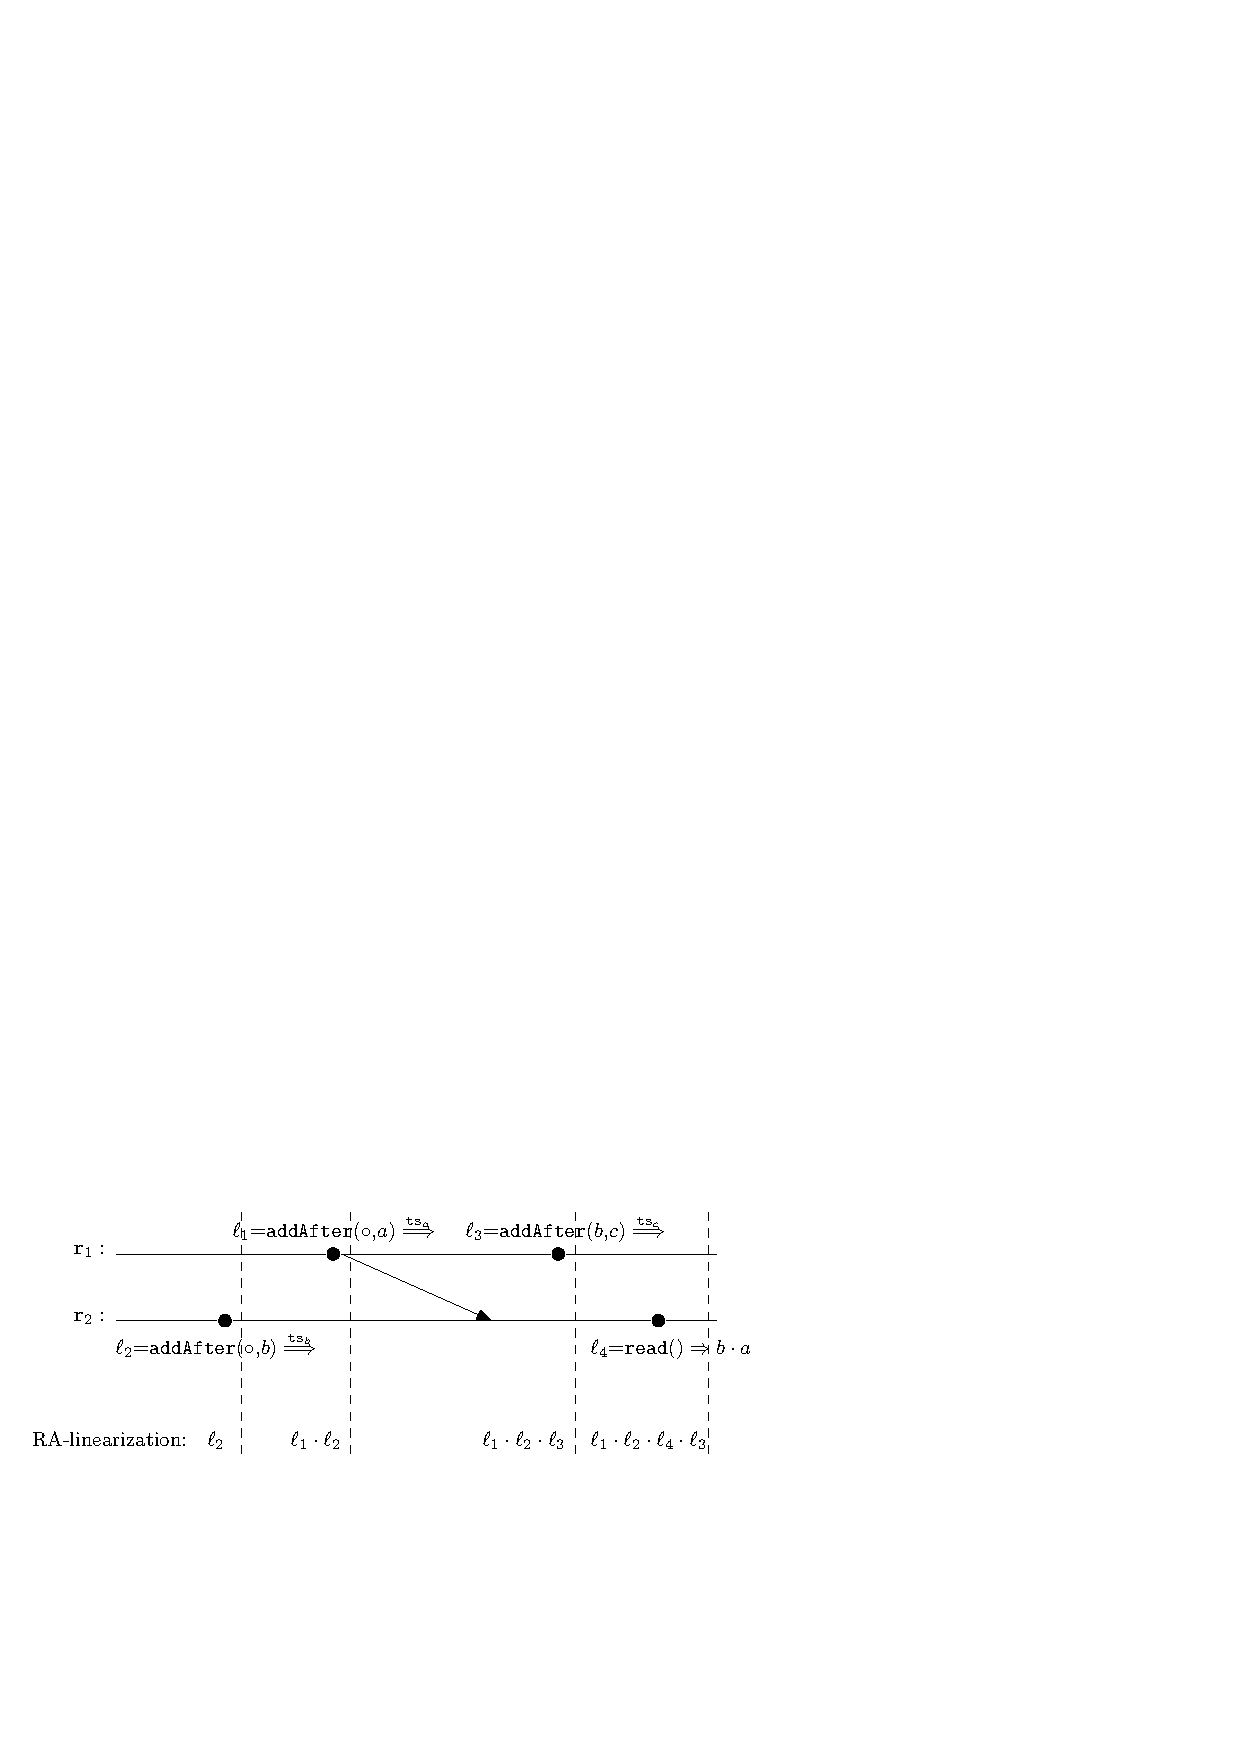
\includegraphics[width=0.6 \textwidth]{figures/RGAHisandLin.pdf}
\vspace{-10pt}
  \caption{A history of RGA and its \crdtlinearization{}.}
  \label{fig:a history of RGA and its RA-linearization}
\end{figure}


\autoref{fig:a history of OR-set, its update-query rewriting, and its RA-linearization} gives a history of OR-set, its query-update rewriting, and its \crdtlinearization{}.

\begin{figure}[t]
  \centering
  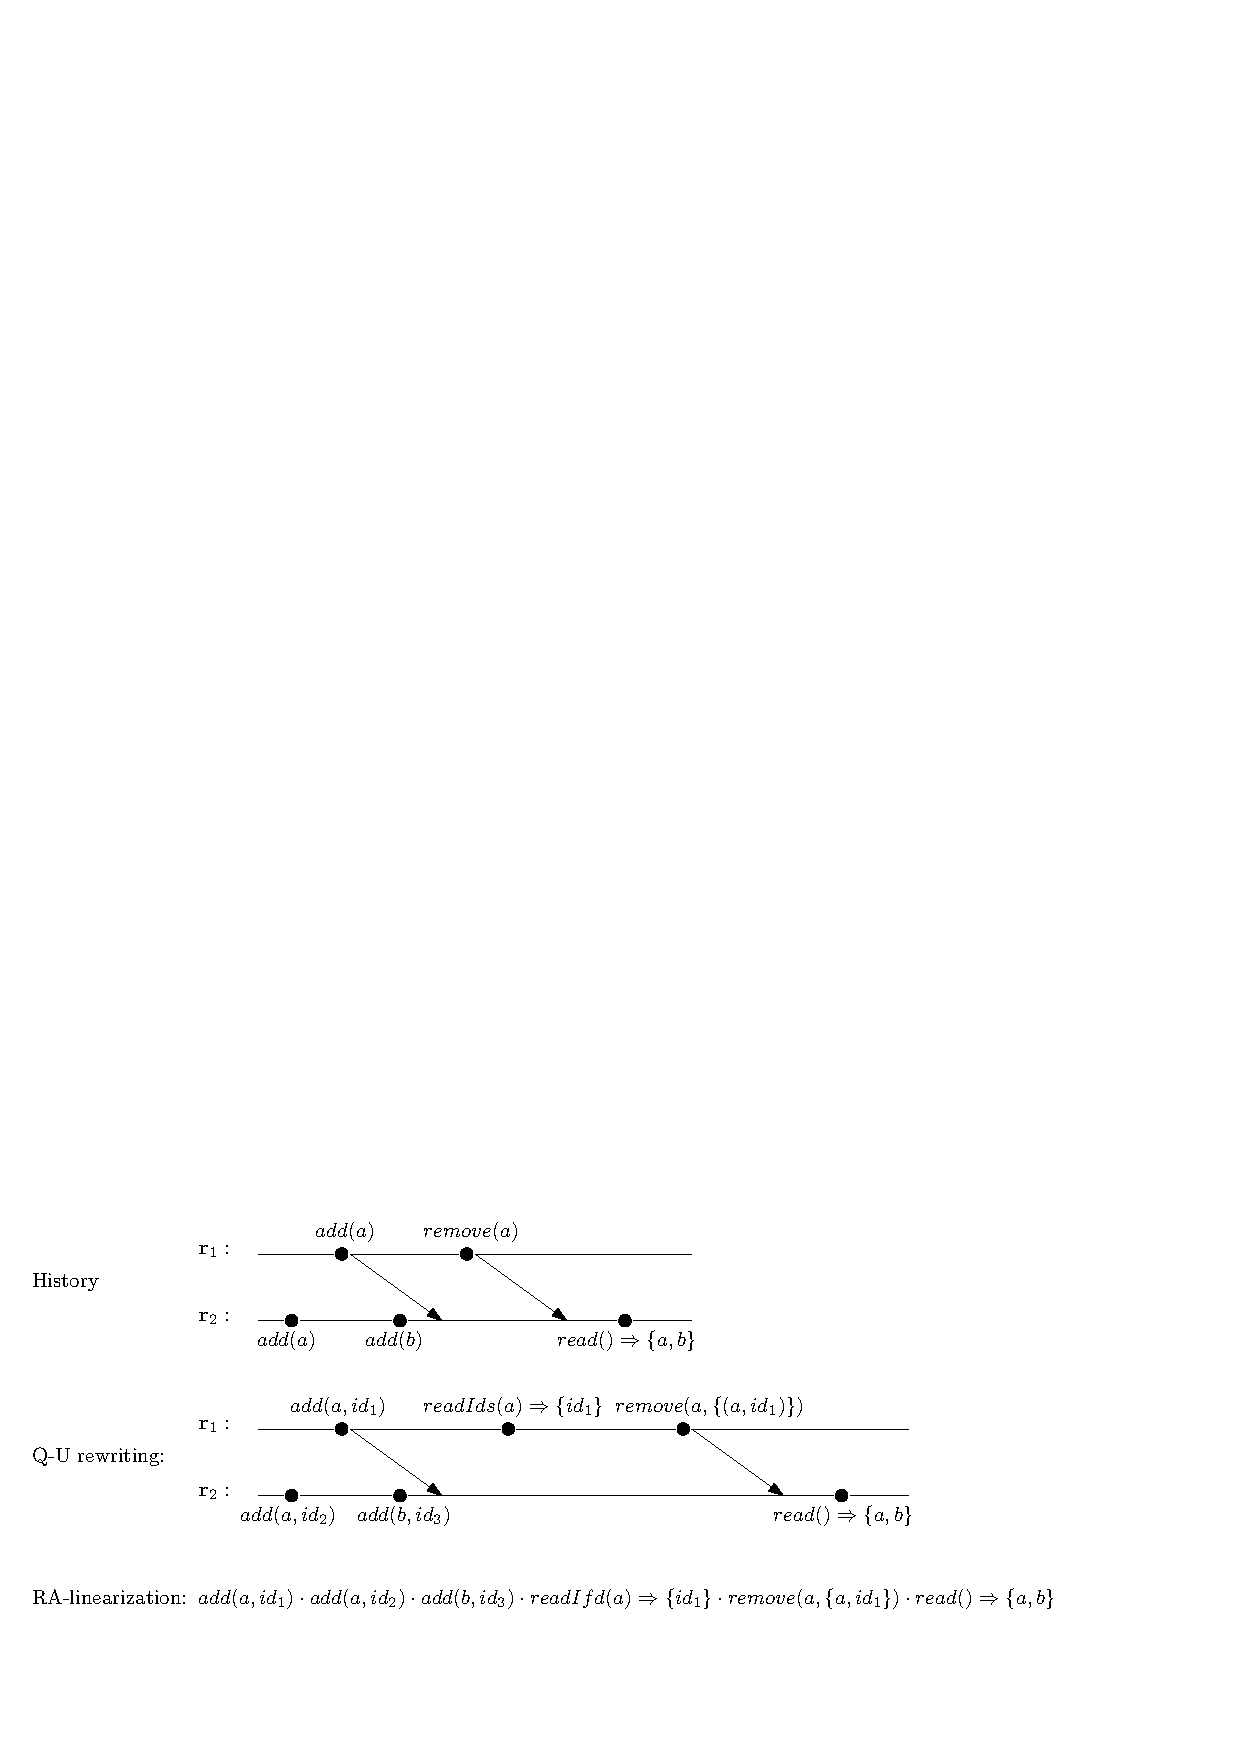
\includegraphics[width=0.8 \textwidth]{figures/ORSetHisRewritingandLin.pdf}
\vspace{-10pt}
  \caption{A history of OR-set, its update-query rewriting, and its \crdtlinearization{}.}
  \label{fig:a history of OR-set, its update-query rewriting, and its RA-linearization}
\end{figure}


\autoref{fig:how refinement mapping works} shows how refinement mapping works. \autoref{fig:how refinement mapping works} (a) shows the case of update labels, \autoref{fig:how refinement mapping works} (b) shows the case of query labels, and \autoref{fig:how refinement mapping works} (c) shows the case of update-query labels.

%Note that, in \autoref{fig:how refinement mapping works} (a) there is a ``gap'' between $\refmap(\sigma)$ and $\refmap(\sigma')$: it may be not the case that $\refmap(\sigma)\xRightarrow{\alabel}\refmap(\sigma')$. Although $\refmap(\sigma')$ should be obtained from $\refmap(\sigma_0)$ by a sequence of the same set of operations as from $\sigma_0$ to $\sigma'$, the order may be different. Such a transition exists for execution-order linearizations, and may not exist for timestamp-order linearizations. What we require here is only that the existence of $\refmap(\sigma')$.

\begin{figure}[t]
  \centering
  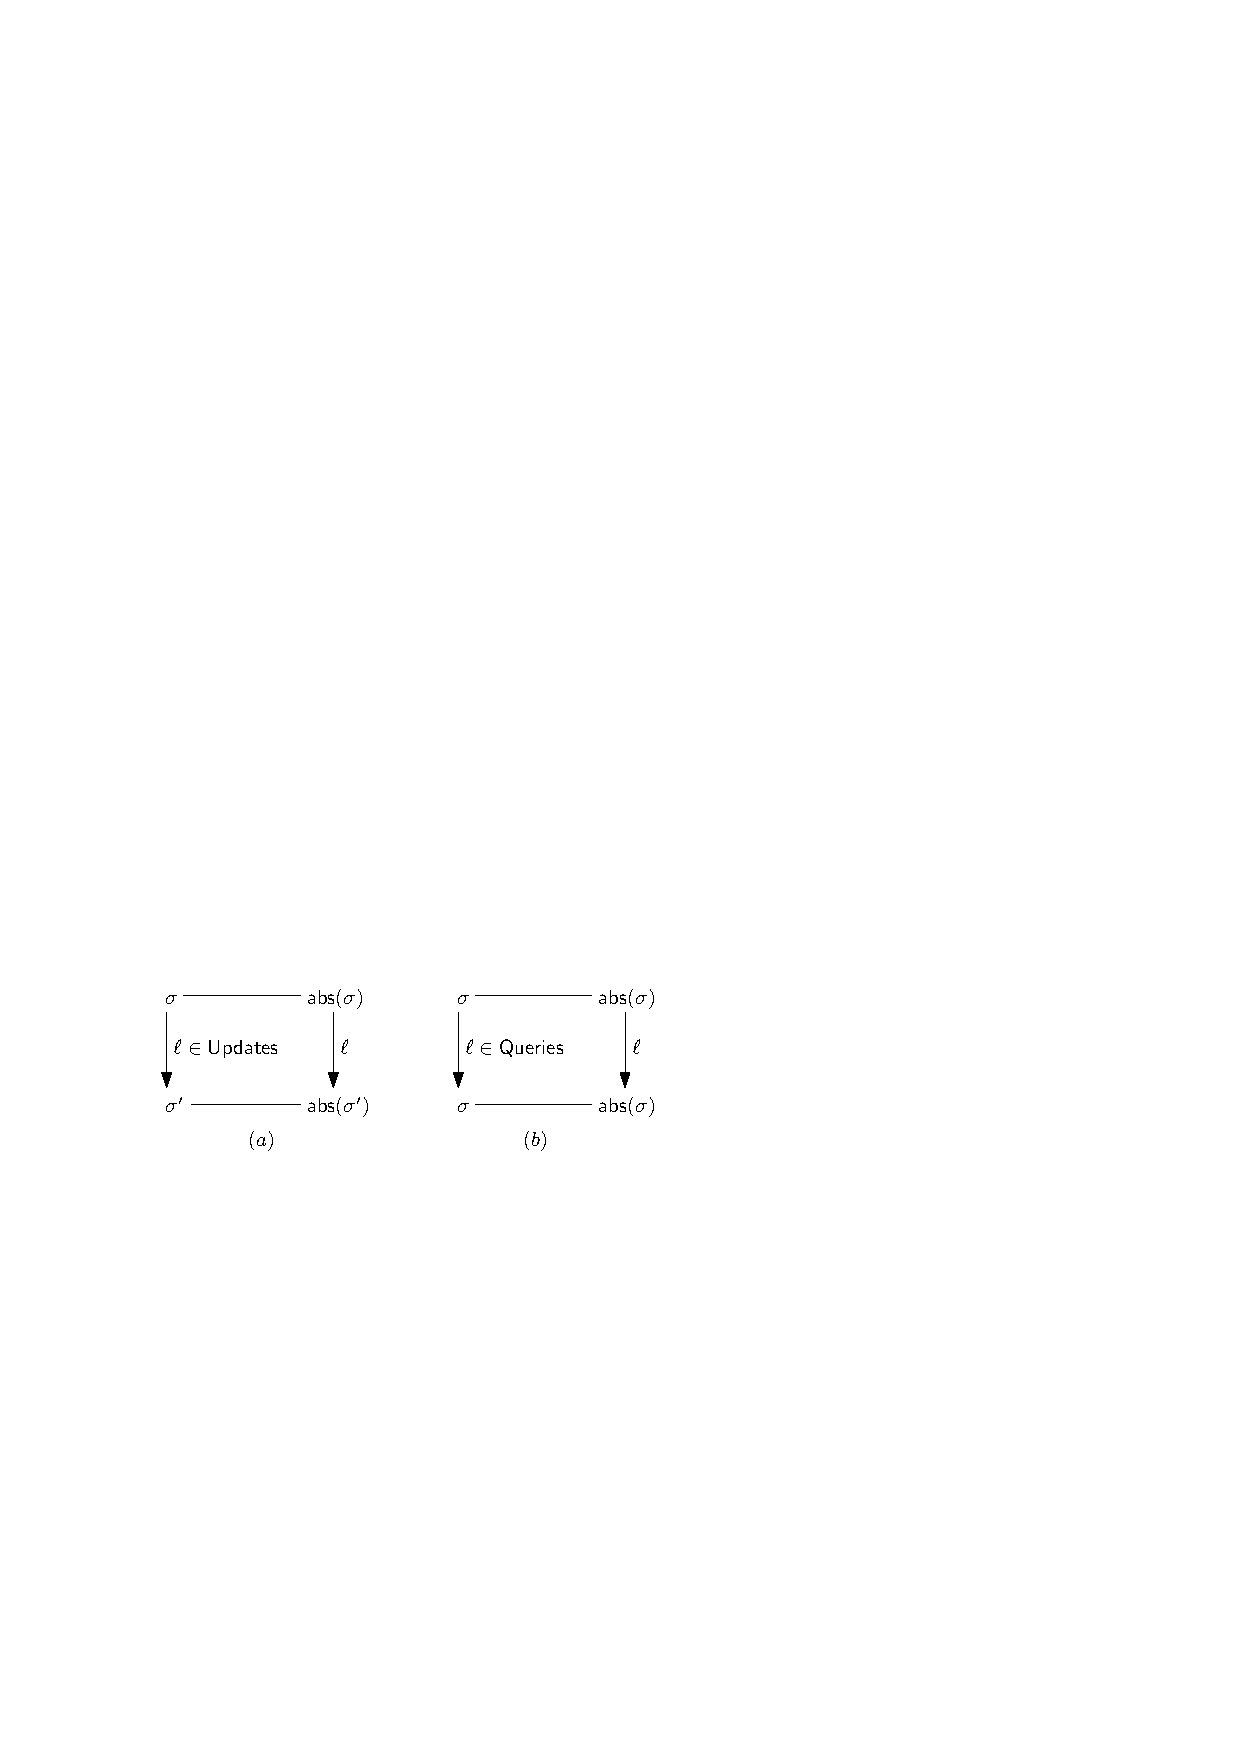
\includegraphics[width=0.8 \textwidth]{figures/RefinementMapping.pdf}
\vspace{-10pt}
  \caption{How refinement mapping works.}
  \label{fig:how refinement mapping works}
\end{figure}



\autoref{fig:an example of refinement mapping of an execution of RGA} gives an example of refinement mapping of an execution of RGA. Here we assume $\ats_a$ and $\ats_b$ is the timestamp of $a$ and $b$ respectively, and the timestamp order be $\ats_a < \ats_b$. Since applying downstream of concurrent operations commute, we take the order of ``increasing timestamp'': $\alabelshort[addAfter]{\circ,a} \cdot \alabelshort[addAfter]{\circ,a} \cdot \alabellong[read]{}{b \cdot a}{}$, and then, according to the refinement mapping, we construct the transitions in sequential specification.

\begin{figure}[t]
  \centering
  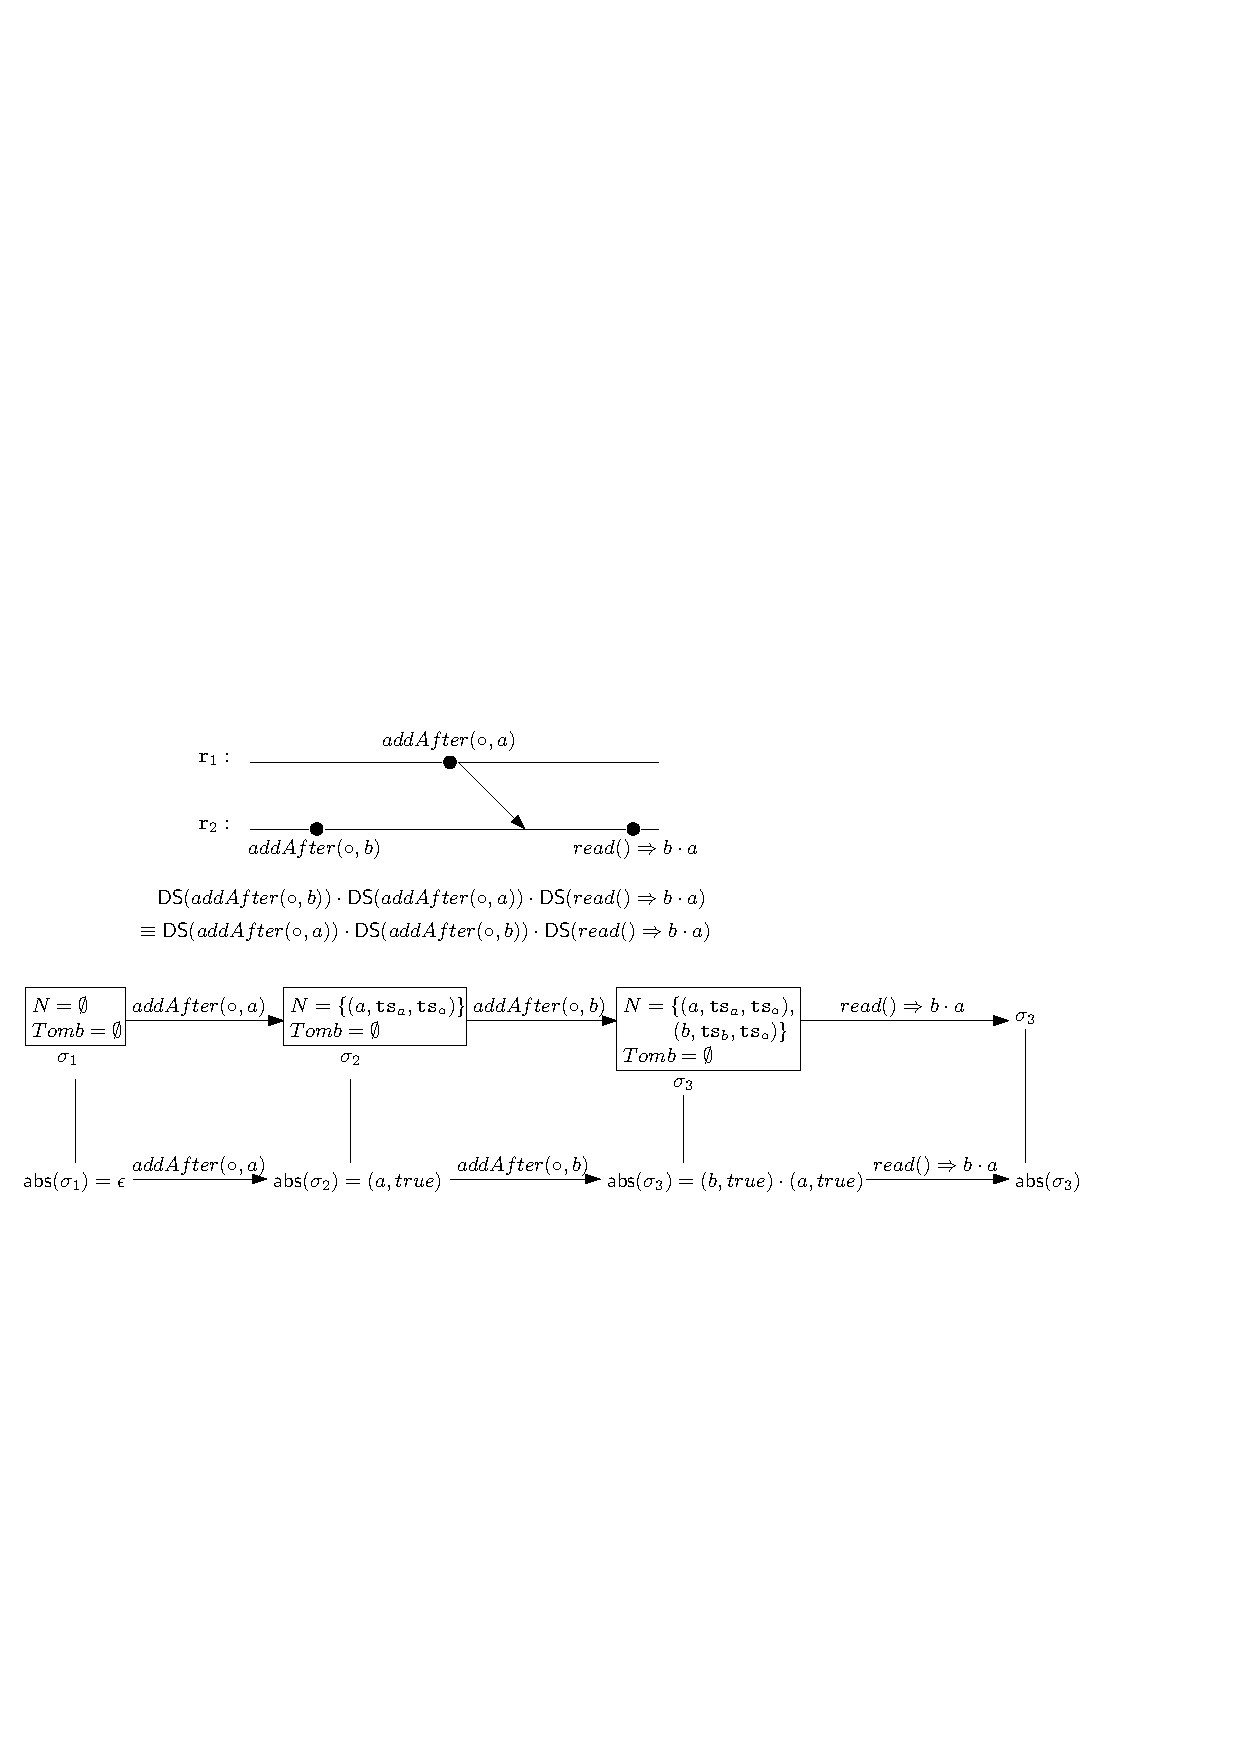
\includegraphics[width=0.85 \textwidth]{figures/RefinementMappingRGA.pdf}
\vspace{-10pt}
  \caption{An example of refinement mapping of an execution of RGA.}
  \label{fig:an example of refinement mapping of an execution of RGA}
\end{figure}



\autoref{fig:an example of refinement mapping of an execution of or-set} gives an example of refinement mapping of an execution of OR-set.

\begin{figure}[t]
  \centering
  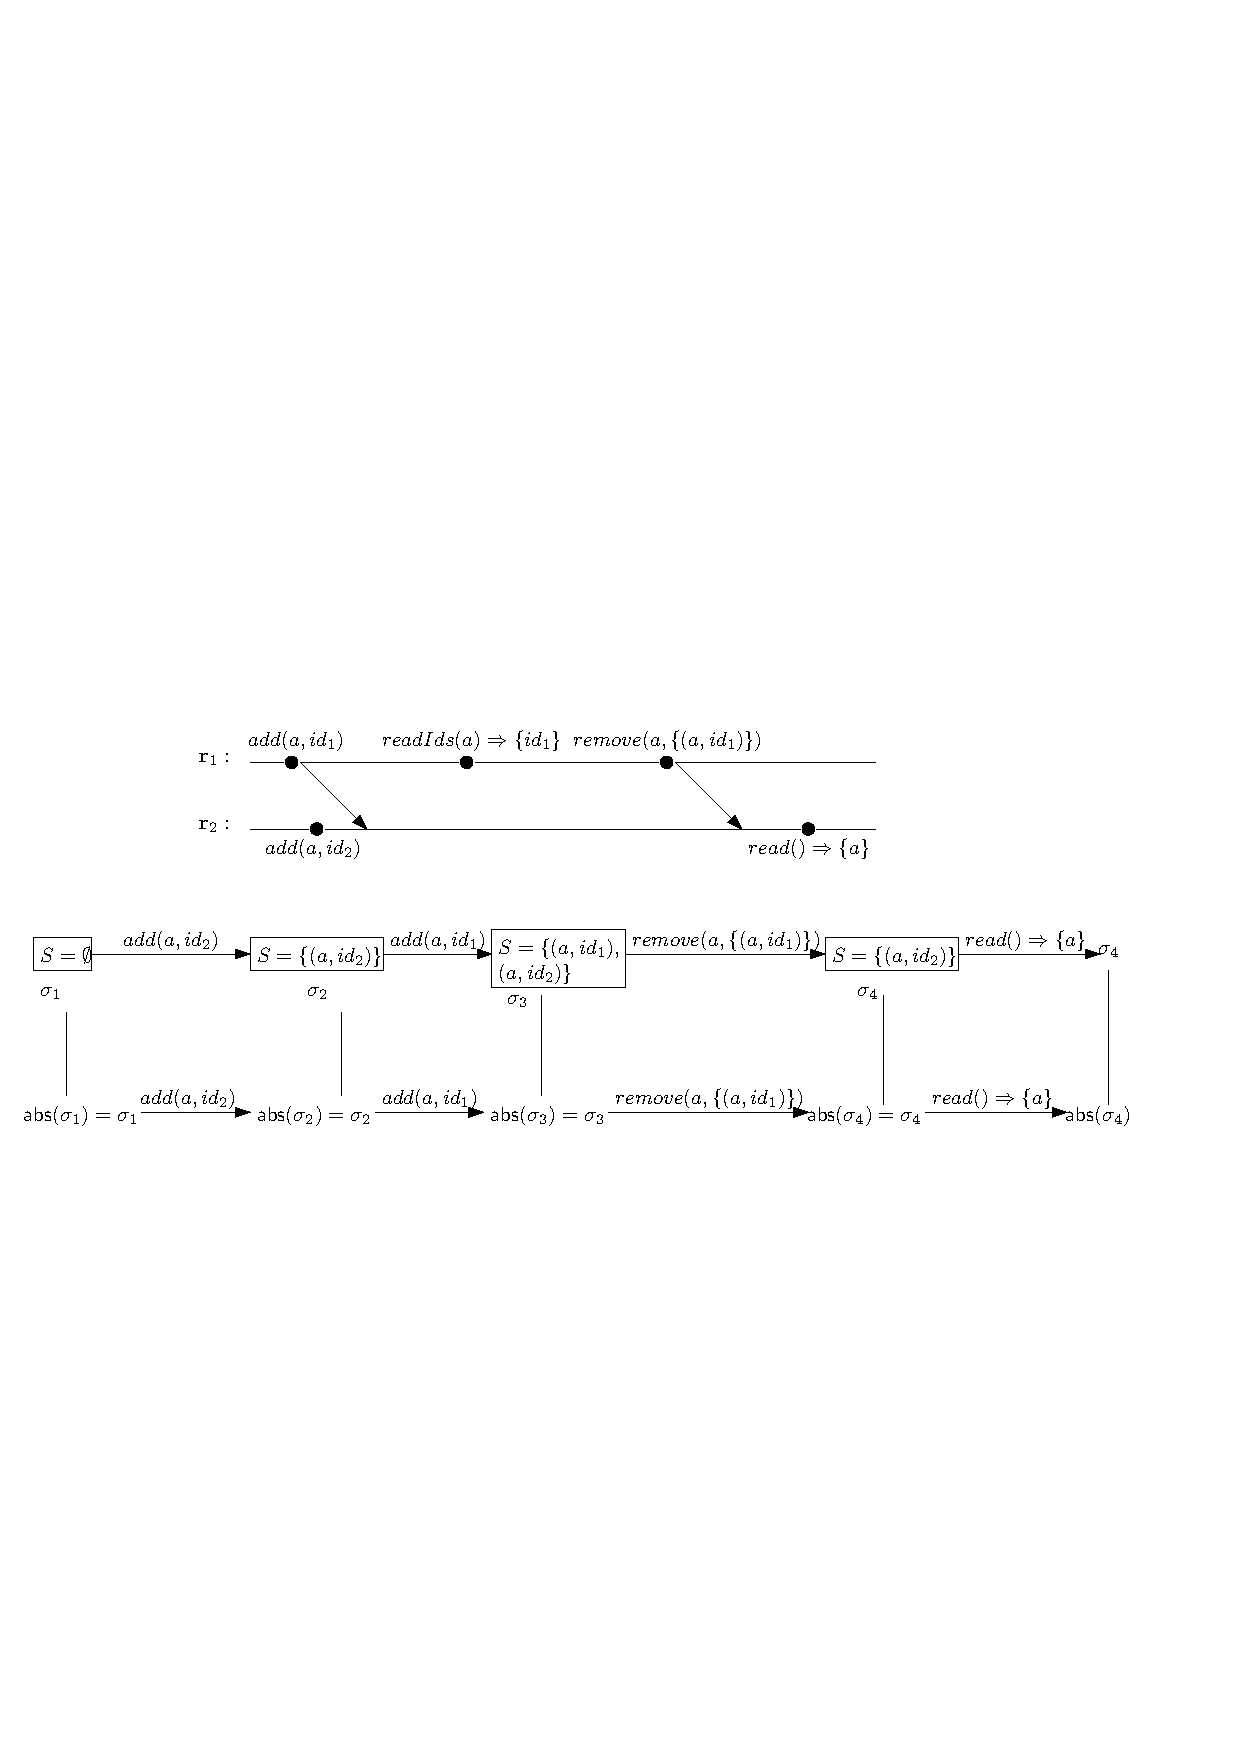
\includegraphics[width=0.85 \textwidth]{figures/RefinementMappingORSet.pdf}
\vspace{-10pt}
  \caption{An example of refinement mapping of an execution of OR-set.}
  \label{fig:an example of refinement mapping of an execution of or-set}
\end{figure}

%Let us consider another possible interface for RGA: $\alabelshort[{\tt addAt}]{a,k}$ puts value $a$ at the $k$-th position of the list, $\alabelshort[{\tt remove}]{a}$ removes a from the list, and $\alabellong[{\tt read}]{}{s}{}$ returns the list $s$. In \autoref{fig:an example that shows RGA with addAt interface is not compositional}, we show an example such that RGA with {\tt addAt} interface is not compositional. Here assume that timestamp order of $a,b$ is $a<b$, and the timestamp of $c,d$ is $c<d$. This history contains operations of two RGA objects $\aobj_1$ and $\aobj_2$, the operations of $\aobj_1$ being represented using blank circles and the operations of $\aobj_2$ using filled circles. The only possible \crdtlinearization{} of $\aobj_1$ is $\aobj_1.\alabelshort[{\tt addAt}]{a,1} \cdot \aobj_1.\alabelshort[{\tt addAt}]{b,2} \cdot \aobj_1.\alabelshort[{\tt remove}]{a}$; since in $\aobj_1.\alabelshort[{\tt addAt}]{a,1} \cdot \aobj_1.\alabelshort[{\tt remove}]{a} \cdot \aobj_1.\alabelshort[{\tt addAt}]{b,2}$, before inserting $b$, the list is $\epsilon$ and $b$ can not be inserted in position $2$. Similarly, the only possible \crdtlinearization{} of $\aobj_2$ is $\aobj_2.\alabelshort[{\tt addAt}]{c,1} \cdot \aobj_2.\alabelshort[{\tt addAt}]{d,2} \cdot \aobj_2.\alabelshort[{\tt remove}]{c}$. However, such two \crdtlinearization{} are not timestamp-order linearizations. Moreover, the two \crdtlinearization{} and the visibility relation berings a cycle.

%In \cite{DBLP:conf/podc/AttiyaBGMYZ16}, they use a more complex interface for RGA and other list implementations: $\alabellong[{\tt addAt}]{a,k}{s}{}, \alabellong[{\tt remove}]{a}{s}{},\alabellong[{\tt read}]{}{s}{}$: $\alabellong[{\tt addAt}]{a,k}{s}{}$ puts value $a$ in position $k$ of the list and returns the updated list $s$, $\alabellong[{\tt remove}]{a}{s}{}$ removes $a$ from the list and returns the updated list $s$, and $\alabellong[{\tt read}]{}{s}{}$ returns the list $s$. Similarly, such interface is not compositional.

%\begin{figure}[t]
%  \centering
%  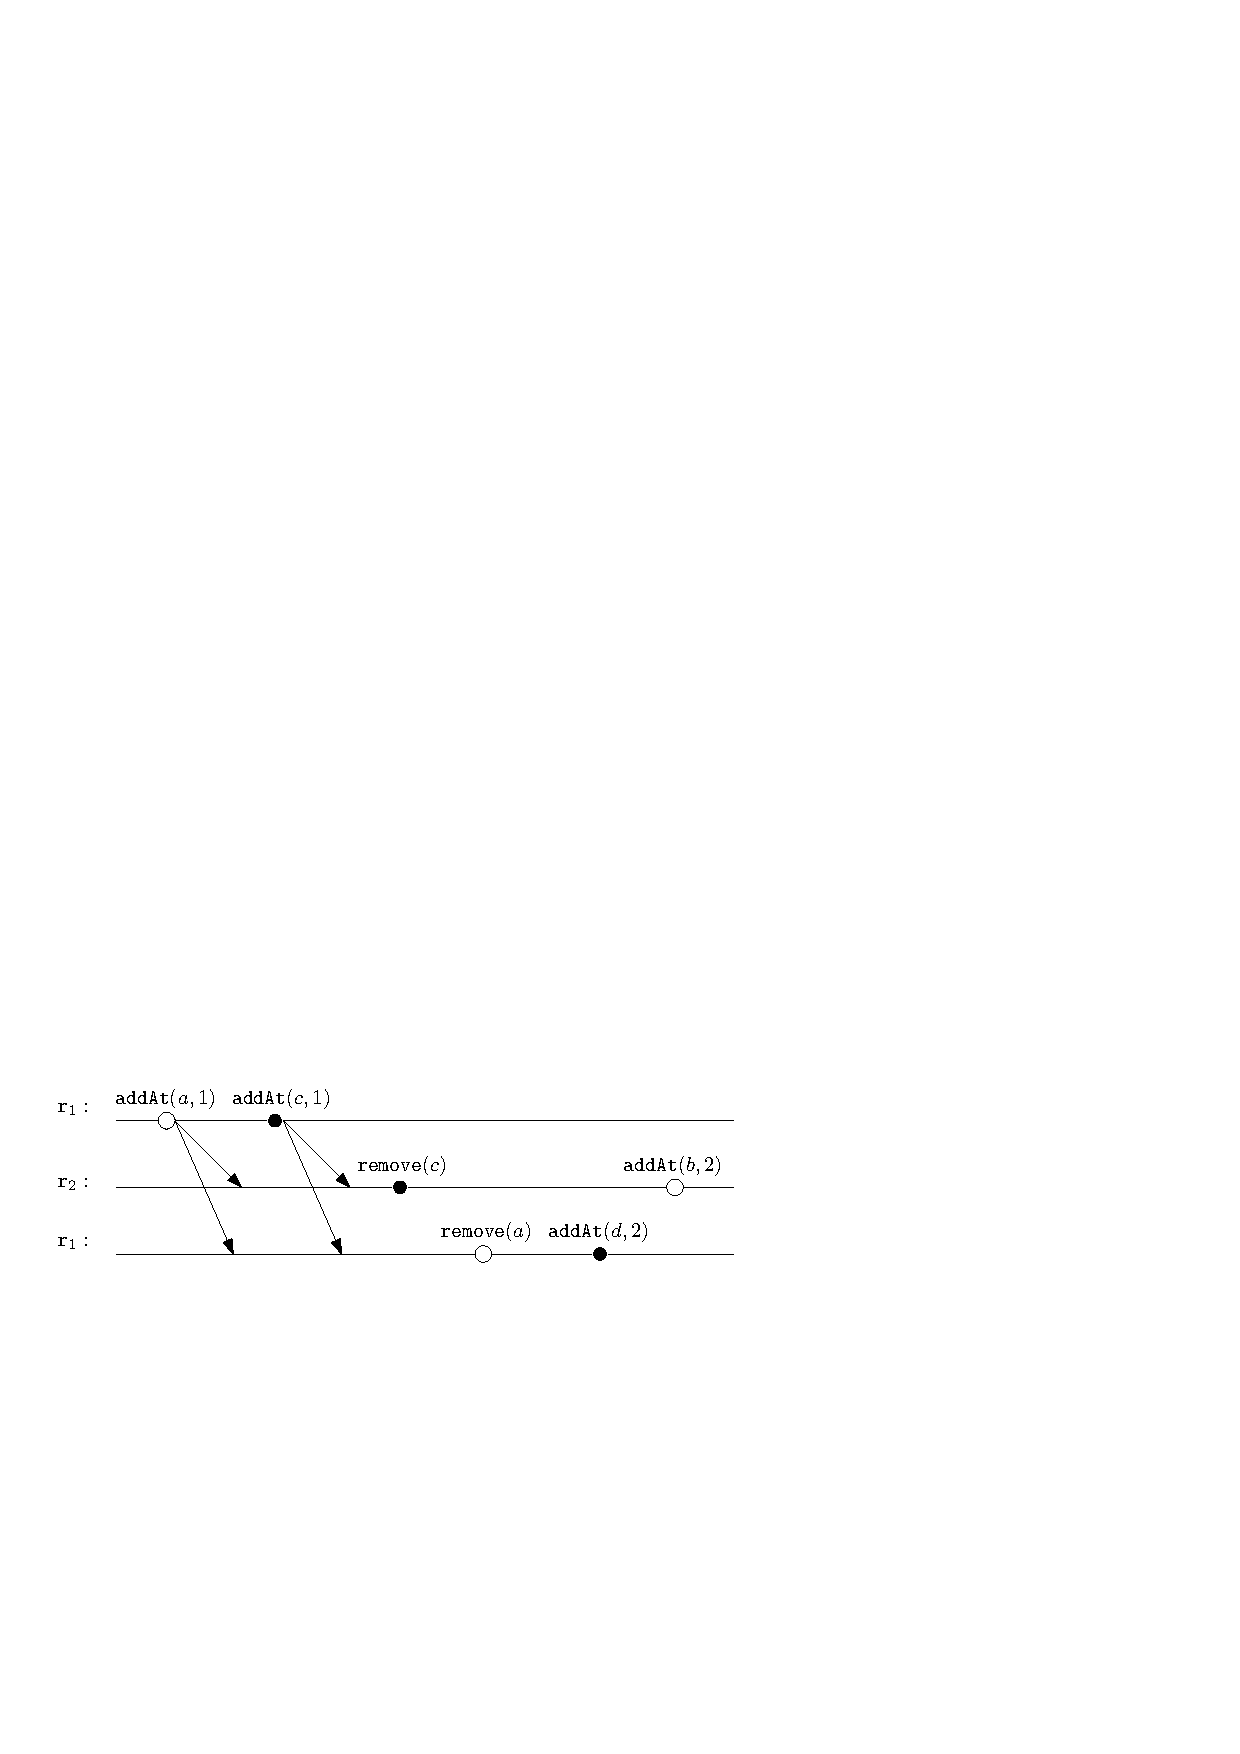
\includegraphics[width=0.85 \textwidth]{figures/RGAwithaddAtnotCompositional.pdf}
%\vspace{-10pt}
%  \caption{An example that shows RGA with {\tt addAt} interface is not compositional.}
%  \label{fig:an example that shows RGA with addAt interface is not compositional}
%\end{figure}



Let us consider another possible interface for RGA: $\alabelshort[{\tt addAt}]{a,k}$ puts value $a$ at the $k$-th position of the list, $\alabelshort[{\tt remove}]{a}$ removes a from the list, and $\alabellong[{\tt read}]{}{s}{}$ returns the list $s$. 

In \autoref{fig:an example that shows RGA with addAt interface is hard to prove}, we shows an example such that the proof of RGA with {\tt addAt} interface is hard to prove. Here assume that timestamp order of $b,c,d,e$ is $b<c<d<e$. Let us call the upper history $h_1$ and the history below $h_2$. The only difference between $h_1$ and $h_2$ is the position of $e$. Both $h_1$ and $h_2$ is \crdtlinearizable{}. However, their \crdtlinearization{} are completely different. We draw the \crdtlinearization{} below the corresponding history. This implies that, the \crdtlinearization{} is no longer timestamp-order linearizations, but something influenced by position. The position $2$ of $e$ in $h_2$ represents that ``the list contains at least one value'', which is essentially a semantics requirement, and it is reasonable to believe that the proof of RGA with {\tt addAt} interface will be much more complex than proving using timestamp-order linearizations.

\begin{figure}[t]
  \centering
  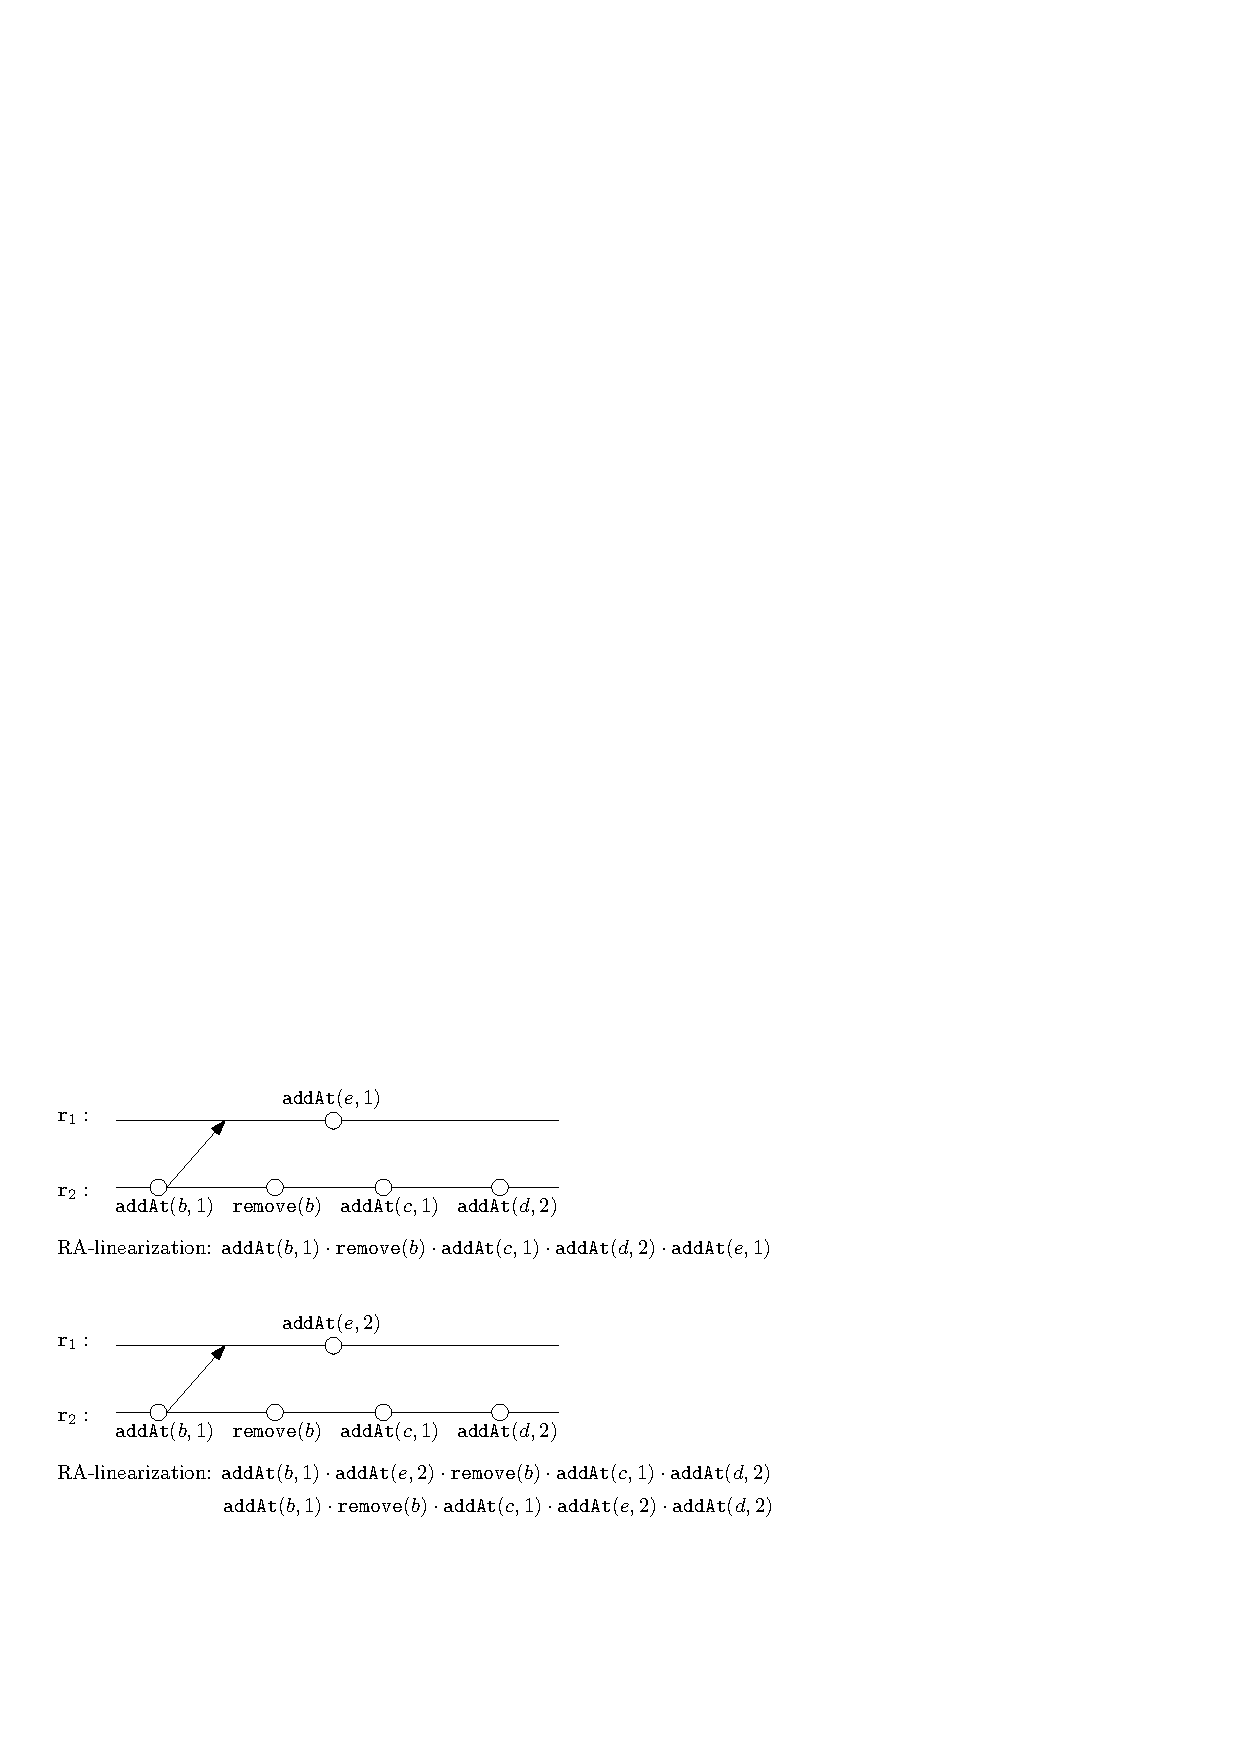
\includegraphics[width=0.7 \textwidth]{figures/RGAwithaddAtisHardtoProve.pdf}
\vspace{-10pt}
  \caption{An example that shows RGA with {\tt addAt} interface is hard to prove.}
  \label{fig:an example that shows RGA with addAt interface is hard to prove}
\end{figure} 


In \autoref{fig:an example that shows RGA with addAt interface is not RAlinearizable}, we shows an example of RGA, it uses {\tt addAt} interface, and is not \crdtlinearizable{}. Here assume that timestamp order of $a,b,c,d,e$ is $a<b<c<d<e$. For easy understanding, we also draw the local state of $\arep_3$ in \autoref{fig:an example that shows RGA with addAt interface is not RAlinearizable}. 

\begin{figure}[t]
  \centering
  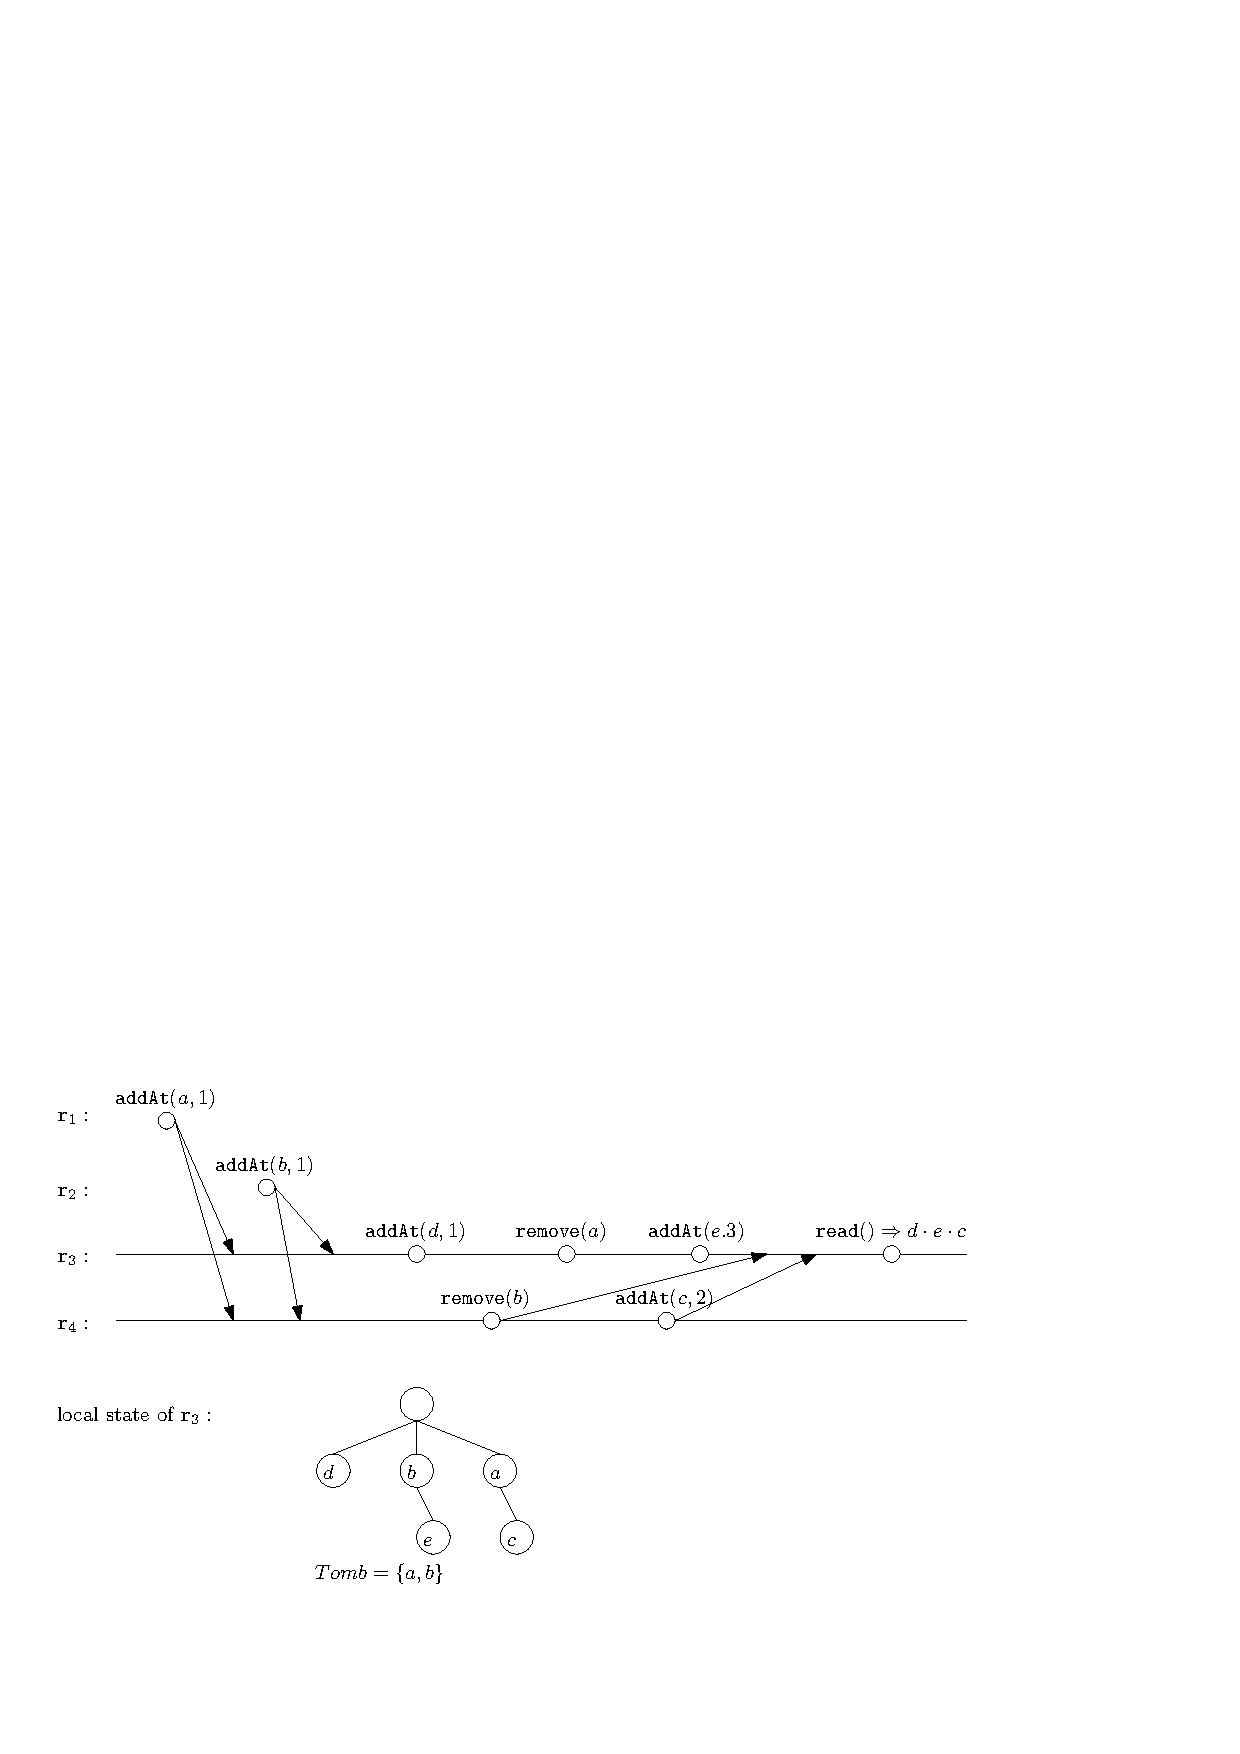
\includegraphics[width=0.7 \textwidth]{figures/RGAwithaddAtNotRALin.pdf}
\vspace{-10pt}
  \caption{An example that shows RGA with {\tt addAt} interface is not \crdtlinearizable{}.}
  \label{fig:an example that shows RGA with addAt interface is not RAlinearizable}
\end{figure} 


Therefore, we can see that, such {\tt addAt} interface is not suitable. In \cite{AttiyaBGMYZ16}, they use a more complex interface for RGA and other list implementations: $\alabellong[{\tt addAt}]{a,k}{s}{}, \alabellong[{\tt remove}]{a}{s}{},\alabellong[{\tt read}]{}{s}{}$: $\alabellong[{\tt addAt}]{a,k}{s}{}$ puts value $a$ in position $k$ of the list and returns the updated list $s$, $\alabellong[{\tt remove}]{a}{s}{}$ removes $a$ from the list and returns the updated list $s$, and $\alabellong[{\tt read}]{}{s}{}$ returns the list $s$. Similarly, such interface has the above drawbacks. 


%The proof of $\mathsf{Refinement}$ relies on a \emph{refinement mapping}~\cite{AbadiL91} between replica states and states of the specification, denoted by $\refmap$. The proof goals require that for any two replica states $\sigma$ and $\sigma'$,
%\begin{enumerate}
%\item If $\sigma'$ is obtained from $\sigma$ by applying a downstream produced by an update $\alabel$: There exists a abstract $\refmap(\sigma')$ that is obtained from $\abstate_0$ by appling the downstreams of the operations in $\alabelset \cup \{ \alabel \}$ in the order defined by $\aseqord$.

%\item if a query $\alabel$ is applied on a state $\sigma$ or it is introduced by a rewriting of a query-update that executes {\tt atSource} on a state $\sigma$, then $\refmap(\sigma)\xRightarrow{\alabel}\refmap(\sigma)$.
%\end{enumerate}

%For the case of execution-order linearizations, the first case can be simplified into

%\begin{enumerate}
%\item if $\sigma'$ is obtained from $\sigma$ by applying a downstream $\delta$ produced by an update $\alabel$, then \mbox{$\refmap(\sigma)\xRightarrow{\alabel}\refmap(\sigma')$}, where $\xRightarrow{\alabel}$ is the transition function of $\Spec$.
%\end{enumerate}

%This simplification relies on proving concurrent operations commute.






























\forget{

\section{Compositionality of Distributed Linearizability}
\label{sec:compositionality of distributed linearizability}

\textblue{
This section should give three results of the form: if $o_1$ is linearizable w.r.t. $S_1$ and $o_2$ is linearizable w.r.t. $S_2$, and ???, then $o_1 \otimes o_2$ is linearizable w.r.t. $S_1\times S_2$ (the 2-object spec defined by interleavings). ??? may be an additional condition, while $\otimes$ is an "operator" for composing two CRDT implementations. Every result will have a different $\otimes$ operator.
\begin{itemize}
\item T0 + T0: ??? = $S_1$ and $S_2$ are $T0$-specs, and $\otimes$ is the trivial composition (the "unsynchronized" product)
\item T1 + T1: ??? = $S_1$ and $S_2$ are $T1$-specs, and $\otimes$ is the "shared counter" composition (the "unsynchronized" product with a restriction on the set of generated histories)
\item T0 + T1: ??? = $S_1$ is a $T_0$ spec, and $S_2$ is a $T1$-spec, and $\otimes$ is the "global causal delivery" composition (the "unsynchronized" product with a restriction on the set of generated histories)
\end{itemize}
Also, we should prove that composing two $T0$, resp., $T1$, specs results in a $T0$, resp., $T1$ spec, and composing a $T0$ with $T1$ results in a $T1$. With this, the extension to sets of objects is straightforward:  compose all $T0$ and independently, all $T1$, then compose the two resulting objects.}


\subsection{Definition of Compositionality}
\label{subsec:definition of compositionality}

The following is the definition of distributed linearizability for multi-object histories.

\begin{definition}[Distributed Linearizability for Multi-object Histories]
\label{definition:distributed linearizability for multi-object histories}
A multi-object history $h$ is \crdtlinearizable{}, if there exists a sequence $\mathit{lin}$, called linearization of $h$, such that

\begin{enumerate}[(i)]
\item The elements of $\mathit{lin}$ is generated from the operations of $h$: each operation $o = (m(a) \Rightarrow b,i,\mathit{obj})$ is transformed into $(m(a) \Rightarrow b,i,S)$ with $S$ set of identifiers of operations of visible to $o$ via $h.\mathit{vis}$.
\item $\mathit{lin}$ is consistent with $h. \mathit{vis}$.
\item For each object $\mathit{obj}$, $h \uparrow_{\mathit{obj}}$ is \crdtlinearizable{}, and $\mathit{lin} \uparrow_{ \mathit{obj} }$ is a \crdtlinearization{} of $h \uparrow_{\mathit{obj}}$.
\end{enumerate}

A set $H$ of multi-object histories are \crdtlinearizable{} w.r.t deterministic sequential specifications, if each of its history is.
\end{definition}

The following is the definition of compositional histories.

\begin{definition}[Compositionality]
\label{definition:compositionality}
A multi-object history $h$ is called compositional, if: $h \uparrow_{\mathit{obj}}$ is distributed linearizable for each object $\mathit{obj}$, if and only if, $h$ is distributed linearizable.
\end{definition}

It is easy to see that, a multi-object history $h$ being distributed linearizable implies that the projection of $h$ into each object is distributed linearizable. When proving compositionality, we only need to consider the opposite direction.




\subsection{T0-Linearizability and T1-Linearizability}
\label{subsec:t0-linearizability and t1-linearizability}

To prove compositional

T0-linearizability is a sub-class of distributed linearizability.

\begin{definition}[t0-linearizability]
\label{definition:t0-ilnearizability}
A single-object history $h$ is t0-linearizable w.r.t a sequential specification $\mathit{spec}$, if each sequence $\mathit{lin}$ shown below is a linearization of $h$ w.r.t $\mathit{spec}$:

\begin{itemize}
\setlength{\itemsep}{0.5pt}
\item[-] Each element $(\ell,i,\mathit{vis}^{-1}(i))$ of $\mathit{lin}$ is generated from an operation $(\ell,i,\_,\mathit{ts})$ of $h$.

\item[-] $\mathit{lin}$ is consistent with $\mathit{vis}$.
\end{itemize}
\end{definition}

To prove t0-linearizability, we introduce the notion of t0-specifications. A specification $\mathit{spec}$ is called t0-specification, if given a history $h$ that is distributed linearizable w.r.t $\mathit{spec}$, then any sequence that is consistent with visibility relation is a linearization of $h$.

The following lemma shows some sequential specifications are t0-specifications. Its proof can be found in Appendix~\ref{subsec:appendix proofs of Lemma several t0-specifications}. Based on this lemma and our proofs in \sectionautorefname~\ref{sec:proving distributed linearizability}, we can see that or-set is t0-linearizable w.r.t $\mathit{OR}$-$\mathit{set}_s$, and counter is t0-linearizable w.r.t $\mathit{counter}_s$.

\begin{restatable}{lemma}{SeveralTZeroSpecifications}
\label{lemma:several t0-specifications}
$\mathit{OR}$-$\mathit{set}_s$, $\mathit{set}_s$ and $\mathit{counter}_s$ are t0-specifications.
\end{restatable}



Given a history $h$, a sequence $\mathit{lin}$ is called a strict time-stamp order candidate of $h$, if for each elements $o_1,o_2$ of $\mathit{lin}$, if the time-stamp of $o_1$ in $h$ is less than that of $o_2$, then, $o_1$ is before $o_2$ in $\mathit{lin}$. T1-linearizability is a sub-class of distributed linearizability.

\begin{definition}[t1-linearizability]
\label{definition:t1-ilnearizability}
A single-object history $h$ is t1-linearizable w.r.t a sequential specification $\mathit{spec}$, if each strict time-stamp order candidiate $\mathit{lin}$ is a linearization of $h$.
\end{definition}

To prove t1-linearizability, we introduce the notion of t1-specifications. A specification $\mathit{spec}$ is called t1-specification, if given a history $h$ that is distributed linearizable w.r.t $\mathit{spec}$, and has a strict time-stamp order candidate as linearization, then any strict time-stamp order candidate is a linearization of $h$.

The following lemma shows some sequential specifications are t1-specifications. Its proof can be found in Appendix~\ref{subsec:appendix proofs of Lemma several t1-specifications}. Based on this lemma and our proofs in \sectionautorefname~\ref{sec:proving distributed linearizability}, we can see that RGA is t1-linearizable w.r.t $\mathit{list}_s^{\mathit{af}}$, and LWW-register is t1-linearizable w.r.t $\mathit{reg}_s$.

\begin{restatable}{lemma}{SeveralTOneSpecifications}
\label{lemma:several t1-specifications}
$\mathit{list}_s^{\mathit{af}}$ and $\mathit{reg}_s$ are t1-specifications.
\end{restatable}


\begin{table}
  \centering
  \begin{tabular}[t]{l|l}
    T0 & $\mathit{OR}$-$\mathit{set}_s$, $\mathit{set}_s$, $\mathit{counter}_s$,  \\
    T1 & $\mathit{list}_s^{\mathit{af}}$, $\mathit{reg}_s$,
  \end{tabular}
\end{table}




\subsection{Composing Several t0-Specifications}
\label{lemma:several t0-specifications can be composed}

The following lemma states that a history of several objects of t0 specifications is compositional. Its proof can be found in Appendix \ref{subsec:appendix proofs of lemma several t0-specifications can be composed}.

\begin{restatable}{lemma}{composingTZero}
\label{lemma:several t0-specifications can be composed}
Given a multi-object history $h$, if each of its object uses a t0-specification, then, $h$ is compositional.
\end{restatable}




\subsection{Composing Several t0-Specifications with One T1-specification}
\label{lemma:composing several t0-specification with one t1-specification}

Composing several t0-specifications with one t1-specification does not hold in general. \autoref{fig:a failed example of composing a multi-value register with a last-write-win register} is a history $h$ that is a failed example of composing a multi-value register with a last-write-win register, where the operations of LWW register are boxed. Here we assume that $\mathit{ts}_1<\mathit{ts}_2$. Since multi-value register is t0-specification and LWW register is t1-specification, we can see that the projection of $h$ into operations of multi-value register is distributed linearization and the only possible linearization is $\mathit{write}(a) \cdot \mathit{write}(b)$, and the projection of $h$ into operations of LWW register is distributed linearization and the only possible linearization is $\mathit{write}(c) \cdot \mathit{write}(d)$. However, $h$ is not distributed linearizable, since there is a a cycle.

\begin{figure}[t]
  \centering
  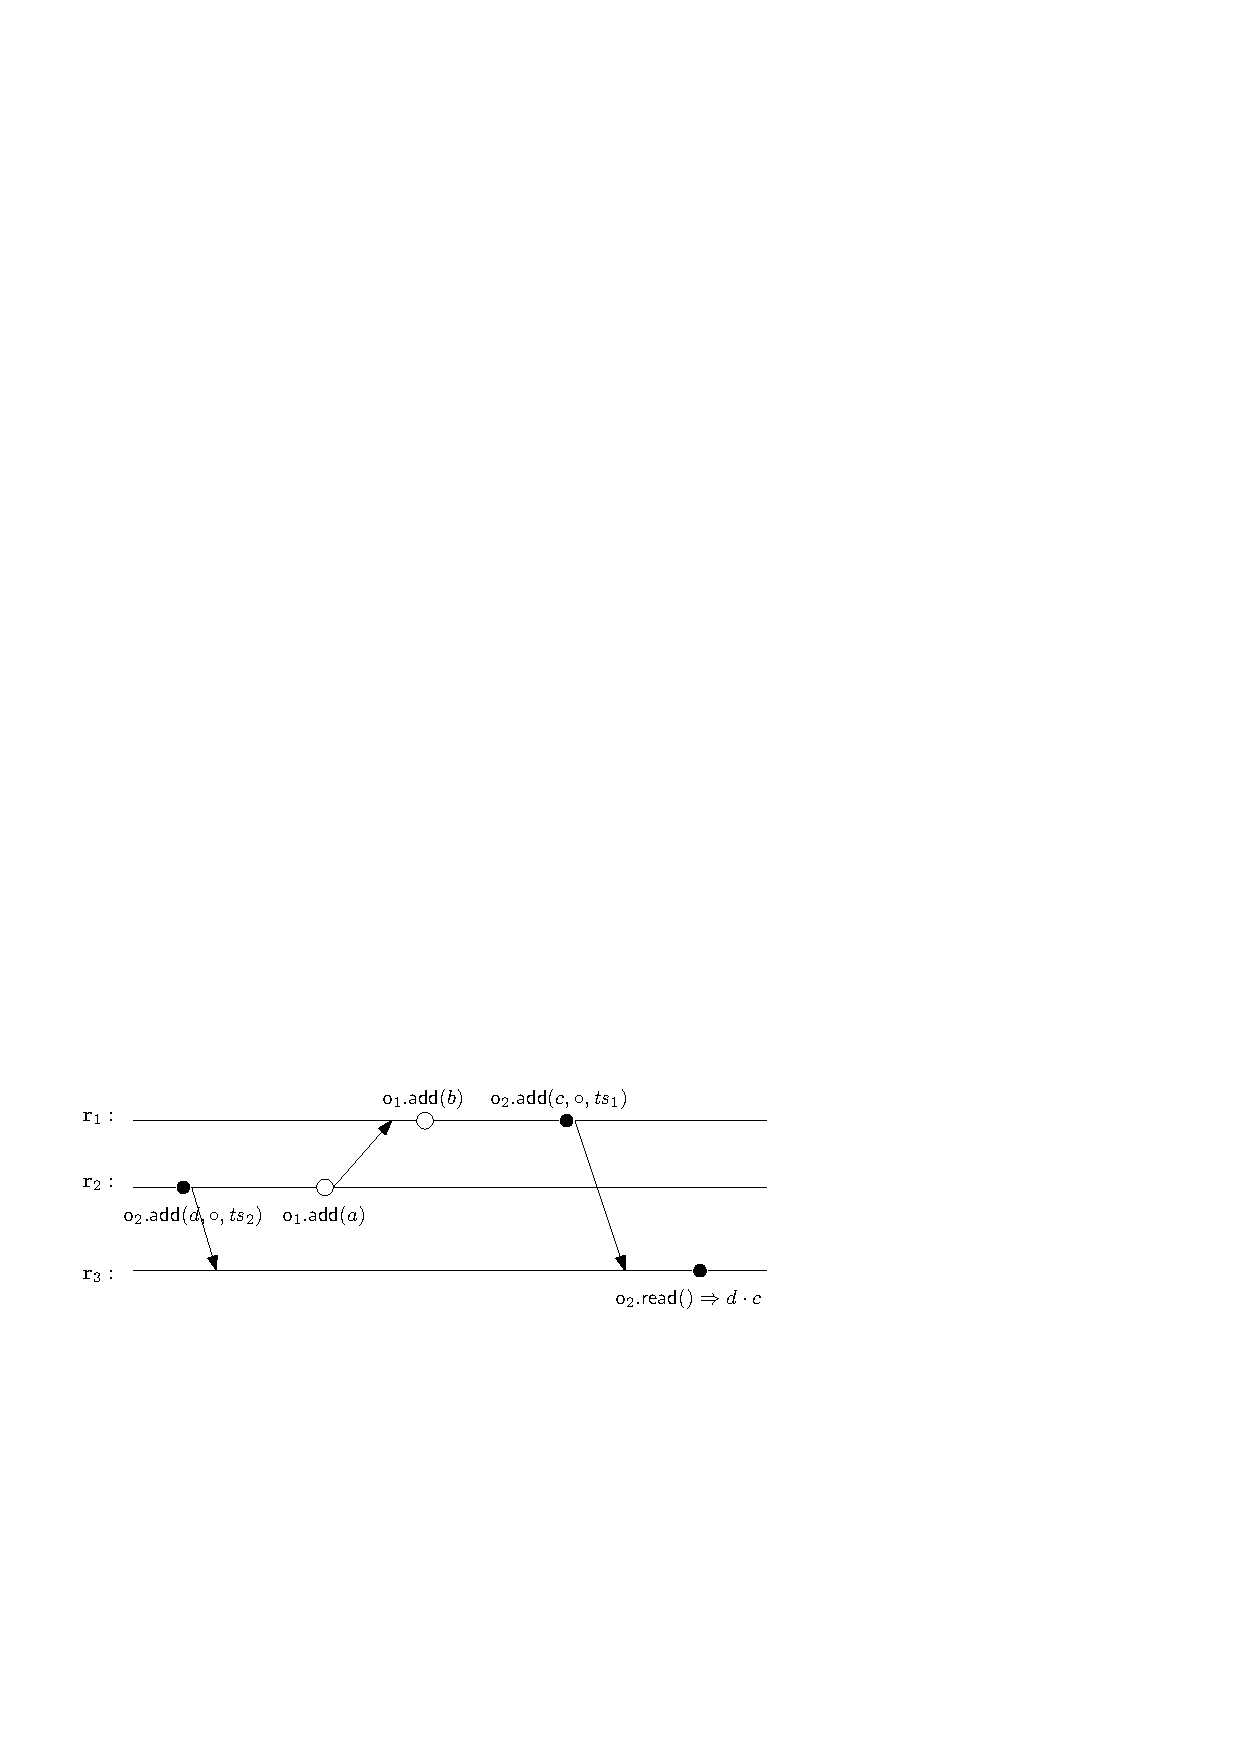
\includegraphics[width=0.6 \textwidth]{figures/MVReg-LWWReg-Nocd.pdf}
\vspace{-10pt}
  \caption{A failed example of composing a multi-value register with a last-write-win register (boxed operations), where $\mathit{ts}_1 < \mathit{ts}_2$.}
  \label{fig:a failed example of composing a multi-value register with a last-write-win register}
\end{figure}

The following lemma states that for a multi-object history, if its object use several t0-specifications and one t1-specification, and its visibility relation is transitive, then, $h$ is compositional. Its proof can be found in Appendix \ref{subsec:appendix proofs of lemma several t0-specifications and one t1-specification can be composed}.

\begin{restatable}{lemma}{composingTZeroAndOneTOne}
\label{lemma:several t0-specifications and one t1-specification can be composed}
Given a multi-object $h$, if its object use several t0-specifications and one t1-specification, and its visibility relation is transitive, then, $h$ is compositional.
\end{restatable}




\subsection{Composing Several t0-Specifications with Several T1-specification}
\label{lemma:composing several t0-specification with several t1-specification}

Composing several t0-specifications with several t1-specification does not hold in general. \autoref{fig:a failed example of composing two last-write-win registers} is a history $h$ that is a failed example of composing two last-write-win registers, where the operations of one LWW register are boxed, and the operations of the other LWW registers are not boxed. Here we assume that $\mathit{ts}_1 < \mathit{ts}_2 < \mathit{ts}_3$, and $\mathit{ts}'_1 < \mathit{ts}'_2$. Since LWW register is t1-specification, we can see that the projection of $h$ into operations of one LWW register is distributed linearization and the only possible linearization is $\mathit{write}(a,\mathit{ts}'_1) \cdot \mathit{write}(b,\mathit{ts}'_2)$, and the projection of $h$ into operations of the other LWW register is distributed linearization and the only possible linearization is $\mathit{write}(c,\mathit{ts}_1) \cdot \mathit{write}(d,\mathit{ts}_2) \cdot \mathit{write}(e,\mathit{ts}_3)$. However, $h$ is not distributed linearizable, since there is a a cycle.

\begin{figure}[t]
  \centering
  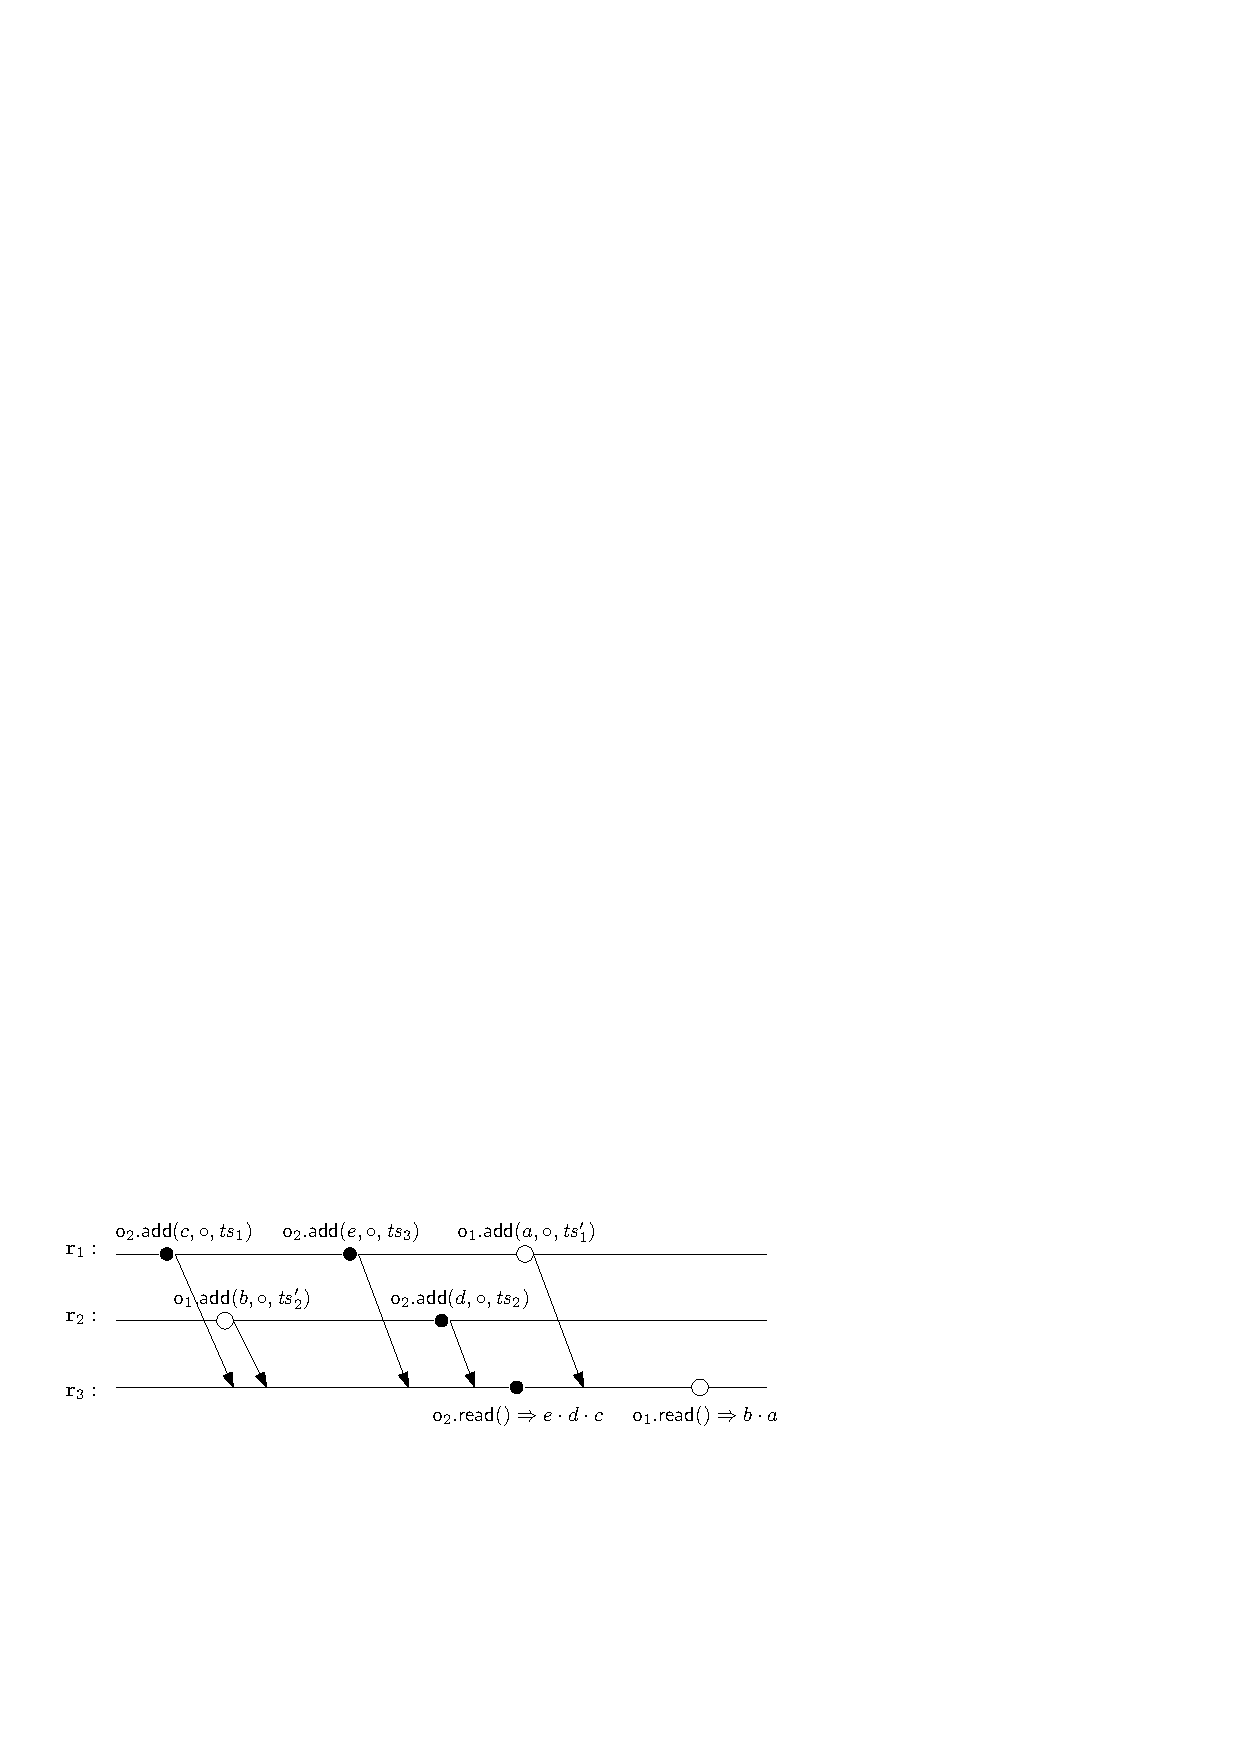
\includegraphics[width=0.7 \textwidth]{figures/LWWReg-LWWReg-NoSTS.pdf}
\vspace{-10pt}
  \caption{A failed example of composing two last-write-win registers (one object is boxed, the other is not), where $\mathit{ts}_1 < \mathit{ts}_2 < \mathit{ts}_3$, and $\mathit{ts}'_1 < \mathit{ts}'_2$.}
  \label{fig:a failed example of composing two last-write-win registers}
\end{figure}


A history $h$ satisfies causal-time-stamp, if: Given operation $o_1,\ldots,o_{\mathit{2k+2}}$ of $h$ that are of objects of t1-specification, if

\begin{itemize}
\setlength{\itemsep}{0.5pt}
\item[-] $(o_2,o_3)$ are of a same object, $\ldots$, $(o_{\mathit{2k}},o_{\mathit{2k+1}})$ are of a same object, $(o_{\mathit{2k+2}},o_1)$ are of a same object,

\item[-] $\mathit{ts}(o_2) < \mathit{ts}(o_2)$, $\ldots$, and $\mathit{ts}(o_{\mathit{2k}}) < \mathit{ts}(o_{\mathit{2k+1}})$,

\item[-] $(o_1,o_2), \ldots, (o_{\mathit{ek+1}},o_{\mathit{2k+2}}) \in \mathit{vis}$.
\end{itemize}

Then, we have $\mathit{ts}(o_1) < \mathit{ts}(o_{\mathit{2k+1}})$.

The following lemma states that for a multi-object history, if its object use several t0-specifications and several t1-specification, and it satisfies causal-time-stamp and its visibility relation is transitive, then, $h$ is compositional. Its proof can be found in Appendix \ref{subsec:appendix proofs of lemma several t0-specifications and several t1-specification can be composed}.

\begin{restatable}{lemma}{composingTZeroAndTOne}
\label{lemma:several t0-specifications and several t1-specification can be composed}
Given a multi-object $h$, if its object use several t0-specifications and several t1-specification, and it satisfies causal-time-stamp and its visibility relation is transitive, then, $h$ is compositional.
\end{restatable}






\subsection{Modified CRDT Implementation}
\label{subsec:modified CRDT implementation}

To ensure composing, we modify t1-algorithms as follows: The system supplies a method called $\mathit{updateGlobalTS}$, which supplies a time-stamp that is updated along the global system. When a method needs to generate new time-stamp, it calls this method to generate new time-stamp, and such process will also update the global time-stamp of this replica. When a method sends a message, the message should contain the current global time-stamp value. When a replica receives a message, it also use the global time-stamp value in message to update its own global time-stamp value. Moreover, the global time-stamp satisfies causal-time-stamp property.

The RGA algorithm after modification is as follows: Here a message contains the current global time-stamp value, and a replica update global time-stamp value is not explicitly written in code. Instead, such processes will be make explicit when constructing the operational semantics.

\begin{lstlisting}[caption={Pseudo-code of the Modified RGA}, captionpos=b,label={lst:modifier rga}]
  payload Ti-Tree N, Set Tomb
  initial N = @|$\emptyset$|@, Tomb = @|$\emptyset$|@

  addAfter(a,b) :
    atSource :
      precondition : b = @|$\circ$|@ or (b != @|$\circ$|@ and (b,_,_) @|$\in$|@ N and b @|$\not\in$|@ Tomb)
      let ts@|$_{\mathtt{a}}$|@ = updateGlobalTS()
      let ts@|$_{\mathtt{b}}$|@ = (b == @|$\circ$|@)?(0,r@|$_{0}$|@):(timestamp of b in N)
    downStream(a, ts@|$_{\mathtt{a}}$|@, ts@|$_{\mathtt{b}}$|@) :
      precondition: b = @|$\circ$|@ or (b != @|$\circ$|@ and (b, ts@|$_{\mathtt{b}}$|@,_) @|$\in$|@ N)
      N = N ts@|$\cup$|@ {(a, ts@|$_{\mathtt{a}}$|@, ts@|$_{\mathtt{b}}$|@)}

  remove(a) :
    atSource :
      precondition : a != @|$\emptyset$|@ and (a,_,_) @|$\in$|@ N and a @|$\notin$|@ Tomb
    downStream(a) :
      precondition : a != @|$\emptyset$|@ and (a,_,_) @|$\in$|@ N
      Tomb = Tomb @|$\cup$|@ {a}

  read() :
    return traverse(N, Tomb)
\end{lstlisting}


The following lemma states that the modified RGA is also t1-linearizable w.r.t $\mathit{list}_s^{\mathit{af}}$, and the modified LWW-register is t1-linearizable w.r.t $\mathit{reg}_s$. Its proof can be found in Appendix \ref{a}.

\begin{restatable}{lemma}{ModifiedRGAandLWWRegStillTOne}
\label{lemma:modified RGA and LWW-register is still t1-linearizable}
$\mathit{list}_s^{\mathit{af}}$ and $\mathit{reg}_s$ are t1-specifications.
\end{restatable}

Lamport's time-stamp is one way to implement global time-stamp, as stated by the following lemma. Its proof can be found in Appendix \ref{a}.

\begin{restatable}{lemma}{LamportTSasGlobalTS}
\label{lemma:lamport time-stamp as global time-stamp}
Lamport's time-stamp satisfies causal-time-stamp.
\end{restatable}








\subsection{Semantics of Multi Objects}
\label{subsec:semantics of multi objects}

When there is multiple objects, we say $(o_1,o_2) \in \mathit{vis}$, if either $(o_1,o_2) \in \mathit{ro}$, or $o_1$ is delivered to the replica of $o_2$ before $o_2$ happens. We consider CTDT implementation of t1-specifications use the time-stamp of Lamport's time-stamp: Each time-stamp is a tuple $(c,r)$ of a counter value $c \in \mathbb{N}$ and a replica identifier $r \in \mathbb{R}$; $(c_1,r_1) < (c_2,r_2)$, if $c_1 < c_2 \vee (c_1 = c_2 \wedge r_1 < r_2)$. To ensure compositionality of multiple objects, the following conditions needs to be satisfied:

\begin{itemize}
\setlength{\itemsep}{0.5pt}
\item[-] Cross-object-causal-delivery (COCD): We extend the notion of causal-delivery into multiple objects. Given two update operations $o_1$ and $o_2$, and assume $o_1$ is visible to $o_2$. Then, for each replica, once it receives $o_2$, it must be the case that $o_1$ has been previously received.

\item[-] Shared-time-stamp (STS): the objects of t1-specifications shares a counter $\mathit{sCtr}$. Each message carries a value of $\mathit{sCtr}$, and when generating new message, the value of $\mathit{sCtr}$ is also considered.
\end{itemize}



Based on shared-time-stamp,



Formally, given a set $\mathit{Objs}$ of objects, its semantics is defined as $\llbracket \mathit{Objs} \rrbracket_{\mathit{op}} = (\mathit{Config},\mathit{config}_0,\Sigma',\rightarrow)$ as in \autoref{fig:the semantics of multiple operation-based CRDT object}.


\begin{figure}[ht]
$\mathit{RState} = \mathit{Objs} \times \mathbb{R} \rightarrow \Sigma$

$\mathit{TState} = \mathbb{MID} \times \mathbb{MSG} \times \mathbb{R} \times \mathit{Objs}$

$\mathit{MsgHB} \subseteq \mathbb{MID} \times \mathbb{MID}$

$\mathit{MsgDel} \subseteq \mathbb{MID} \times \mathbb{R}$

$\mathit{Config} = \mathit{RState} \times \mathit{TState} \times \mathit{MsgHB} \times \mathit{MsgDel}$, $\mathit{config}_0 \in \mathit{Config}$.

$\Sigma' = \mathit{do}(\mathit{Objs} \times \mathbb{M} \times \mathbb{D} \times \mathbb{D} \times \mathbb{R} \times \mathbb{MID}) \cup \mathit{do}(\mathit{Objs} \times \mathbb{M} \times \mathbb{D} \times \mathbb{D} \times \mathbb{R}) \cup \mathit{receive}(\mathit{Objs} \times \mathbb{MID} \times \mathbb{R})$

\begin{itemize}
\setlength{\itemsep}{0.5pt}
\item[] $\begin{array}{l c}
   \bigfrac{
   \begin{array}{c}
     R(x,r) = \sigma, (x,r).\mathit{do}(\sigma,m,a) = (\sigma',b,\mathit{msg}), \mathit{msg} \neq \emptyset, \mathit{unique}(\mathit{mid}), \\
     S_1 = \{ (\mathit{mid}',\mathit{mid}) \vert (\mathit{mid'},r) \in \mathit{MsgDel} \}, S_2 = \{ (\mathit{mid}',\mathit{mid}) \vert \mathit{mid}' \in T, \mathit{mid}' \ is \ of \ replica \ r \}
   \end{array}}
     {(R,T,\mathit{msgHB},\mathit{MsgDel}) {\xrightarrow{\mathit{do}(x,m,a,b,r,\mathit{mid})}} (R[(x,r):\sigma'], T \cup \{ (\mathit{mid},\mathit{msg},r,x) \}, (\mathit{MsgHB} \cup S_1 \cup S_2)^*,\mathit{MsgDel})}
\end{array}$

\item[] $\begin{array}{l c}
   \bigfrac{
   \begin{array}{c}
     R(x,r) = \sigma, (x,r).\mathit{do}(\sigma,m,a) = (\sigma',b,\emptyset)
   \end{array}}
     {(R,T,\mathit{msgHB},\mathit{MsgDel}) {\xrightarrow{\mathit{do}(x,m,a,b,r)}} (R[(x,r):\sigma'], T \cup \{ (\mathit{mid},\mathit{msg},r) \}, \mathit{MsgHB},\mathit{MsgDel})}
\end{array}$

\item[-] $\begin{array}{l c}
   \bigfrac{
   \begin{array}{c}
      R(x,r) = \sigma, (x,r).\mathit{receive}(\sigma,\mathit{msg}) = \sigma', (\mathit{mid},\mathit{msg},r',x) \in T, r \neq r', \\
      (\mathit{mid},r) \notin \mathit{MsgDel}, \mathit{mid} \ is \ minimal \ w.r.t \ \mathit{MsgHB} \ among \ \{ \mathit{mid}' \vert (\mathit{mid}',r) \notin \mathit{MsgDel} \}
   \end{array}}
     {(R,T,\mathit{msgHB},\mathit{MsgDel}) {\xrightarrow{\mathit{receive}(x,\mathit{mid},r)}} (R,T,\mathit{MsgHB},\mathit{MsgDel} \cup \{ (\mathit{mid},r) \} )}
\end{array}$
\end{itemize}
\caption{The definition of semantics of $\llbracket \mathit{Objs} \rrbracket_{\mathit{op}}$}
\label{fig:the semantics of multiple operation-based CRDT object}
\end{figure}




$R$ is now a function from object and replica identifier to local state. Message and action also record its object. $\mathit{MsgHB}$ and $\mathit{MsgDel}$ now record the relation between messages of multiple objects. In each transition rule of \autoref{fig:the semantics of multiple operation-based CRDT object}, we deal with each object according to its CRDT implementations. Similarly, a sequence $l$ of actions is an execution of $\llbracket \mathit{Objs} \rrbracket_{\mathit{op}} = (\mathit{Config},\mathit{config}_0,\Sigma',\rightarrow)$, if there exists $(R,T,\mathit{MsgHB},\mathit{MsgDel}) \in \mathit{Config}$, such that $\mathit{config}_0 {\xrightarrow{ l }} (R,T,\mathit{MsgHB},\mathit{MsgDel})$. The semantics of $\mathit{Objs}$ is defined as the set of executions of $\llbracket \mathit{Objs} \rrbracket_{\mathit{op}}$.





A configuration $(R,T,\mathit{MsgHB},\mathit{MsgDel})$ is a snapshot of distributed system. $R$ gives the local state of each replica, and $T$ gives the set of messages that has been generated. Let $\mathbb{MID}$ be the set of message identifiers of message content. A message is a tuple $(\mathit{mid},\mathit{msg},r)$, where $\mathit{mid} \in \mathbb{MID}$ is the identifier, $\mathit{msg} \in \mathbb{MSG}$ is the message content, and $r$ is the original replica of message. $\mathit{MsgHB}$ is used to record the happen-before relation between messages: two messages $(\mathit{mid}_1,\mathit{mid}_2) \in \mathit{MsgHB}$ represents that the operation of $\mathit{mid}_1$ happens before the operation of $\mathit{mid}_2$. $\mathit{MsgDel}$ is used to record the message delivery relation between messages: $(\mathit{mid},r) \in \mathit{MsgDel}$ represents that message $\mathit{mid}_1$ has already been delivered to replica $r$. $\mathit{MsgHB}$ and $\mathit{MsgDel}$ are used to ensure message delivery requirements. $\mathit{config}_0$ is the initial configuration, which maps each replica into the initial local state, has no message, and with a empty happen-before relation and a empty message delivery relation.


Each element of $\Sigma'$ is called an action. $\rightarrow \in \mathit{Config} \times \Sigma' \times \mathit{Config}$ is the transition relation and describes a single step of distributed systems. The first rule in \autoref{fig:the semantics of a operation-based CRDT object} describes replica $r$ performs a update operation $m(a) \Rightarrow b$ and generates a message with message content $\mathit{msg}$. Here $\mathit{unique}$ is a function that ensures $\mathit{mid}$ be a fresh message identifier. We insert message identifier $\mathit{mid}$ into the happen-before relation and keeps the happen-before relation be transitive. The second rule describes replica $r$ performs a query operation $m(a) \Rightarrow b$ and thus does not generate message. Since no message is generated, the $\mathit{MsgHB}$ and $\mathit{MsgDel}$ tuples remain the same. The third rule describes delivery of a message to a replica $r$ other than its origin replica $r'$. By $(\mathit{mid},r) \notin \mathit{MsgDel}$, we ensure that $\mathit{mid}$ has not been previously delivered to replica $r$, and thus, each message be delivered to each replica at most once. By $\mathit{mid}$ being minimal w.r.t $\mathit{MsgHB}$ among $\{ \mathit{mid}' \vert (\mathit{mid}',r) \notin \mathit{MsgDel} \}$, we always choose a minimal element w.r.t $\mathit{MsgHB}$ among operations not been delivered to a replica, and thus, ensures causal-delivery.



\subsection{Proving in Multi-Objects Semantics}
\label{subsec:proving in multi-object semantics}


The formation of CRDT in this semantics is changed as follows,

The CRDT proved distributed linearizable are still distributed linearizable in this new semantics.
}

%%% Local Variables:
%%% mode: latex
%%% TeX-master: "draft"
%%% End:
